\documentclass[journal]{IEEEtran}

% ---- IEEE Transactions on Intelligent Transportation Systems ----
\usepackage[T1]{fontenc}
\usepackage[utf8]{inputenc}
\usepackage{cite}
\usepackage{graphicx}
\usepackage{amsmath}
\usepackage{amsfonts}
\usepackage{amssymb}
\usepackage{booktabs}
\usepackage{multirow}
\usepackage{makecell}
\usepackage{nicefrac}
\usepackage{xcolor}
\usepackage{subcaption}
\usepackage{xspace}
\usepackage{microtype}
\usepackage{url}
\usepackage[hidelinks]{hyperref}

% Custom macros
\newcommand{\method}{EgoPed\xspace}
\newcommand{\eg}{e.g.,\xspace}
\newcommand{\ie}{i.e.,\xspace}
\newcommand{\etal}{\textit{et al.}\xspace}
\newcommand{\uparrowb}{\textbf{$\uparrow$}}
\newcommand{\downarrowb}{\textbf{$\downarrow$}}
\newcommand{\TODO}[1]{{\textcolor{red}{{#1}}}} % TODOs in red

\begin{document}

\title{Ego-Conditioned Pedestrian Body Motion Generation\\via Latent Diffusion with Full-Sequence Ego Conditioning}

\author{Erik Sch\"utz\TODO{, Co-Author, and Co-Author}% 
\thanks{\TODO{Affiliations, e-mail addresses, and funding acknowledgement.}}%
\thanks{\TODO{Manuscript received Month DD, YYYY; revised Month DD, YYYY.}}}

\markboth{IEEE Transactions on Intelligent Transportation Systems}%
{Sch\"utz \MakeLowercase{\textit{et al.}}: Ego-Conditioned Pedestrian Body Motion Generation via Latent Diffusion}

\maketitle


\begin{abstract}
We introduce \method, a system that generates 3D full-body pedestrian motion conditioned on vehicle ego trajectories from autonomous driving data.
Existing pedestrian motion synthesis relies on text descriptions or action labels, ignoring the driving context that shapes how a person walks, stops, or reacts.
We condition a Motion Latent Diffusion model on ego odometry by exposing the denoiser to all 196 per-timestep ego tokens rather than a pooled summary, through a frozen, alignment-pretrained ego encoder.
On a combined nuScenes, Waymo and AVA benchmark, full-sequence conditioning improves FID by \textbf{40\%} over the strongest pooled baseline (5.620~$\to$~3.392), at equal denoiser capacity and against that baseline's best seed.
We then show that this metric cannot carry the conditioning claim: separately trained unconditional models reach FID 3.24, and 1.43 under interaction-aware sampling --- the best marginal we measure --- while remaining ego-blind at chance-level retrieval.
Grounding the claim instead in per-condition measurements on a scene-disjoint held-out split, full-sequence conditioning leads on trajectory error (ADE 2.46~$\to$~2.36\,m) and on the coupling between generated stopping decisions and the vehicle (0.28~$\to$~0.33), both significant under a paired bootstrap.
Ablations show the frozen encoder is critical and the attention mechanism is not; interaction-aware sampling improves the marginal (FID 2.67--2.88 over two seeds) but not per-condition fidelity.
Finally, a reference-free audit of the pose labels --- one canonical skeleton for every pedestrian, and feet that essentially never plant --- bounds what FID can mean on this benchmark.
\end{abstract}

\begin{IEEEkeywords}
Pedestrian behaviour modelling, human motion synthesis, denoising diffusion models, autonomous driving, vehicle--pedestrian interaction, generative model evaluation, motion capture data quality.
\end{IEEEkeywords}

%----------------------------------------------------------------------
\section{Introduction}
%----------------------------------------------------------------------

\IEEEPARstart{G}{enerating} realistic pedestrian body motion is a critical capability for autonomous vehicle (AV) simulation.
Simulation pipelines require diverse, plausible pedestrian behaviour --- walking, turning, stopping, reacting to traffic --- to stress-test perception and planning before deployment, and especially for the long tail of close-range encounters that are unsafe or impractical to collect on the road.
The intelligent-transportation literature has long established that this behaviour is coupled to the vehicle: the ego vehicle's speed, trajectory and proximity all influence whether a pedestrian crosses, waits, accelerates or turns~\cite{camara2021pedmodels2}, and benchmarks such as JAAD~\cite{rasouli2017jaad} and PIE~\cite{rasouli2019pie} annotate exactly that dependence.
Those benchmarks, however, predict discrete events --- will the pedestrian cross? --- and the models built on them output a label or a ground-plane trajectory~\cite{alahi2016sociallstm,salzmann2020trajectron,gu2022mid}, not an articulated body.

Full-body human motion synthesis has meanwhile advanced rapidly, driven by text-conditioned diffusion models~\cite{chen2023mld,tevet2023mdm,zhang2022motiondiffuse,guo2024momask}.
These systems are context-agnostic in precisely the way an AV simulator cannot afford: a pedestrian crossing a street is generated identically whether a vehicle is approaching at 50~km/h or standing still.
The \emph{ego-conditioned} setting that joins the two literatures --- generating full 3D body motion conditioned on the vehicle's own trajectory --- is largely unexplored.
Existing work either generates 2D trajectory distributions only~\cite{mao2023led}, or uses ego context as scene conditioning without 3D body synthesis~\cite{feng2024unitraj}, while spatially controlled motion models~\cite{karunratanakul2023gmd,xie2024omnicontrol} constrain the generated person directly rather than conditioning on a second, independently moving agent.

This paper addresses ego-conditioned \emph{full-body} pedestrian motion synthesis.
We build on Motion Latent Diffusion (MLD)~\cite{chen2023mld}, which compresses 263D HumanML3D body motion into a compact latent space and denoises within it, but replace the text conditioning with vehicle ego trajectory.
The key architectural question is: \emph{how should the ego trajectory be injected into the denoiser?}

We study two families of conditioning mechanisms:
\begin{itemize}
\item \textbf{Pooled conditioning}: The ego trajectory is encoded by a transformer encoder and mean-pooled to a single 256D token, which is concatenated alongside the time embedding in the denoiser's self-attention. This gives the denoiser a coarse summary of the ego trajectory but no temporal resolution.
\item \textbf{Full-sequence conditioning}: The ego trajectory is encoded to a full 196-token sequence, which is concatenated with the latent tokens and jointly self-attended at each denoising step. This exposes every denoising step to the full ego trajectory, enabling temporally fine-grained conditioning.
\end{itemize}

Our main finding is that full-sequence conditioning dramatically outperforms pooled conditioning.
\method achieves \textbf{FID = 3.392} versus the pooled baseline's 5.620 under a unified evaluation pipeline — a 40\% improvement with the same denoiser capacity, whose best checkpoint occurs \emph{earlier} in training (epoch 3399 vs.\ 4399), so the gain does not come from additional compute. Adding interaction-aware training-data sampling improves our best system further to FID = 2.880.
The full-sequence denoiser can attend to specific moments in the ego trajectory rather than a coarse average, producing motion that more closely follows the ground truth distribution.

A secondary but equally important finding concerns the ego encoder's training regime.
\method uses a \emph{frozen} ego encoder — pretrained to align mean-pooled ego trajectories with VAE motion latents, then fixed during diffusion training.
We ablate this choice with Unfrozen, which unfreezes the encoder and allows it to co-adapt with the denoiser.
Unfrozen consistently \emph{underperforms} \method on the distributional metrics at every evaluated checkpoint: FID worsens by 50\%, R-Precision@1 drops by 36\%, and MultiModality collapses by 34\%.
We show that this occurs because the unfrozen encoder specializes to discriminative, per-condition representations that over-constrain generation diversity — consistent with the frozen-encoder paradigm in image generation (frozen CLIP in Stable Diffusion~\cite{rombach2022sd}, adapters on frozen backbones in IP-Adapter~\cite{ye2023ipadapter} and ControlNet~\cite{zhang2023controlnet}).

Our contributions are:
\begin{enumerate}
\item The first system to generate full 3D HumanML3D body motions conditioned on vehicle ego odometry, trained on AVA, nuScenes~\cite{caesar2020nuscenes}, and Waymo~\cite{sun2020waymo} data.
\item A negative result with methodological consequences: FID ranks \emph{marginals}, not conditioning. Separately trained unconditional models --- one on the standard recipe, which matches our full-sequence model (3.241 vs.\ 3.392), and one on the interaction-sampling recipe, which beats every conditional model in the paper (1.43) --- sit at chance on every conditioning metric. We supply the controls (trajectory ADE/FDE, a behavioral stop/walk probe, and an information ladder over conditioning signals from 0 to 6.09 bits) that do separate the two.
\item A demonstration that full-sequence temporal conditioning achieves a 40\% FID improvement over single-token pooled conditioning under a unified evaluation pipeline (non-overlapping confidence intervals, 3 replications), and --- more importantly --- that it also leads on per-condition metrics computed on a scene-disjoint held-out split (trajectory ADE and the coupling of stopping decisions to the vehicle), which is what distinguishes conditioning from marginal fit. The gain is robust to the attention mechanism.
\item A reference-free audit of the pseudo-ground-truth poses over the full extraction of 14{,}172 sequences, quantifying what the labels do and do not support: the root trajectories are reliable, while body shape is a single canonical template and the feet do not plant. We show the artifact is already present in the motion VAE, and that correcting the labels removes it from reconstruction, which scopes the fix as relabelling rather than an added training loss.
\item An ablation showing that frozen ego encoders are critical for generative diversity in ego-conditioned motion: unfreezing collapses MultiModality by 34\% and worsens FID by 50\%, though it slightly improves mean trajectory error --- a trade we quantify rather than assert away.
\item A design recommendation: frozen ego encoder + full-sequence conditioning (\method) is the best-conditioned architecture for this task, and the one we recommend deploying; interaction-aware sampling is an orthogonal data-side choice that trades per-condition fidelity for marginal realism.
\end{enumerate}

%----------------------------------------------------------------------
\section{Related Work}
\label{sec:related}
%----------------------------------------------------------------------

\subsection{Pedestrian Behaviour Modelling for Automated Driving}

Modelling how pedestrians behave around vehicles is a long-standing concern in intelligent transportation. Camara \etal survey the area in two parts, separating low-level sensing, detection and tracking~\cite{camara2021pedmodels1} from high-level models of pedestrian decision-making and vehicle--pedestrian interaction~\cite{camara2021pedmodels2}. The dominant experimental paradigm is video-based and predicts discrete events. JAAD~\cite{rasouli2017jaad} annotates crossing behaviour together with its situational context; PIE~\cite{rasouli2019pie} adds large-scale intention labels alongside ego-vehicle sensor readings, making the vehicle state an explicit input. Kotseruba \etal~\cite{kotseruba2021benchmark} re-evaluate pedestrian action prediction under a common protocol and find that reported gains are strongly sensitive to evaluation design and to the base rate of the predicted event.

We share the domain but change the output. Rather than classifying whether a pedestrian will cross, we synthesise the full articulated body motion conditioned on the vehicle trajectory. The protocol lesson of~\cite{kotseruba2021benchmark} transfers directly, and is one motivation for the per-condition controls in Sections~\ref{sec:adefde} and~\ref{sec:behavior}: a metric that looks decisive can be insensitive to exactly the effect it is being used to argue for.

\subsection{Pedestrian and Agent Trajectory Prediction}

A large literature predicts pedestrians as points on the ground plane. Social LSTM~\cite{alahi2016sociallstm} introduced neural social pooling; Social GAN~\cite{gupta2018socialgan} made the prediction explicitly multi-modal; Social-STGCNN~\cite{mohamed2020stgcnn} replaced recurrence with a spatio-temporal graph. Trajectron++~\cite{salzmann2020trajectron} incorporates heterogeneous agents and dynamic feasibility, and AgentFormer~\cite{yuan2021agentformer} models social and temporal dimensions jointly with attention. Goal-conditioned formulations predict an endpoint first and the path second~\cite{mangalam2020pecnet,mangalam2021ynet}. Diffusion has since become a standard generator in this space, with MID~\cite{gu2022mid} treating prediction as progressive denoising of indeterminacy and LED~\cite{mao2023led} accelerating sampling through a learned initialiser. On the vehicle side, MTR~\cite{shi2022mtr} couples global intention localisation with local refinement, and UniTraj~\cite{feng2024unitraj} studies cross-dataset generalisation across nuScenes, Argoverse~2 and Waymo Open Motion. Rudenko \etal~\cite{rudenko2020survey} and Karle \etal~\cite{karle2021survey} survey the human and vehicle branches respectively.

All of these predict root position. Our root-trajectory evaluation in Section~\ref{sec:adefde} deliberately borrows their metrics --- average and final displacement error, reported as min-of-$K$ --- so that the conditioning question can be asked on the axis this literature has already validated. The difference is that our model must additionally produce body articulation, and, as Section~\ref{sec:posequality} shows, the two components of the output are not of equal quality.

\subsection{Human Motion Synthesis and Latent Diffusion}

Generating 3D human motion from a high-level specification progressed from action labels~\cite{petrovich2021actor} to free-form language~\cite{petrovich2022temos}, supported by the HumanML3D corpus and its 263-dimensional redundant motion representation~\cite{guo2022humanml3d}, which we adopt. Denoising diffusion~\cite{ho2020ddpm}, with deterministic DDIM sampling~\cite{song2021ddim} and classifier-free guidance~\cite{ho2022cfg}, now dominates the area: MDM~\cite{tevet2023mdm} and MotionDiffuse~\cite{zhang2022motiondiffuse} denoise raw motion, while MLD~\cite{chen2023mld} moves the process into the latent space of a motion VAE~\cite{kingma2014vae}, following latent diffusion in images~\cite{rombach2022sd}. MLD is our backbone: we retain its frozen VAE, transformer denoiser~\cite{vaswani2017attention} and sampler, and replace the text condition with vehicle ego odometry. Alternative generators include discrete token prediction~\cite{zhang2023t2mgpt}, generative masked modelling~\cite{guo2024momask}, motion-as-language formulations~\cite{jiang2023motiongpt}, retrieval augmentation~\cite{zhang2023remodiffuse}, and the reuse of a pretrained motion diffusion model as a generative prior for downstream tasks~\cite{shafir2024priormdm}.

Closest in spirit to our conditioning problem is spatially controlled motion generation. GMD~\cite{karunratanakul2023gmd} guides generation with ground-plane trajectory constraints, and OmniControl~\cite{xie2024omnicontrol} controls any joint at any time through a combination of spatial guidance and a learned control branch. These methods constrain the generated human directly: the control signal specifies where that person's own body should be. Our condition differs in kind. The ego trajectory belongs to a \emph{different} agent, and never determines the output --- it shapes a distribution over plausible reactions. This distinction is what makes conditioning so difficult to verify here, and is the reason a distributional score alone cannot establish it.

\subsection{Interaction- and Scene-Conditioned Motion}

Motion conditioned on external context is usually conditioned on static geometry. PROX~\cite{hassan2019prox} resolves pose ambiguity using scene constraints, SAMP~\cite{hassan2021samp} generates stochastic scene-aware movement and interaction, HUMANISE~\cite{wang2022humanise} pairs language with 3D scenes, and TRUMANS~\cite{jiang2024trumans} scales dynamic human--scene interaction data and modelling. For multi-agent settings, InterGen~\cite{liang2024intergen} generates two interacting people with mutual attention. Our setting sits between these: the conditioning agent is dynamic rather than static geometry, but unlike two-person interaction it is observed and fixed, which permits a simpler asymmetric design in which the ego trajectory enters the denoiser as a fixed token sequence.

\subsection{Frozen Encoders in Conditional Generative Models}

A recurring pattern in conditional image generation is that frozen conditioning encoders preserve generative diversity better than jointly fine-tuned ones. Stable Diffusion~\cite{rombach2022sd} keeps its text encoder frozen; IP-Adapter~\cite{ye2023ipadapter} and ControlNet~\cite{zhang2023controlnet} attach conditioning adapters to a frozen generative backbone. Conversely, methods that fine-tune the generative stack for condition fidelity, such as DreamBooth~\cite{ruiz2023dreambooth}, are known to trade away diversity and require explicit prior-preservation regularisation to recover it. Our freeze-versus-unfreeze ablation (Section~\ref{sec:h6}) supplies direct evidence for the same phenomenon in motion generation, and further shows that the degradation is not uniform across metrics: unfreezing improves mean trajectory error while collapsing per-condition diversity.

\subsection{Pseudo-Ground-Truth Motion Labels}

Large-scale driving datasets~\cite{caesar2020nuscenes,sun2020waymo,wilson2021argoverse2} provide vehicle odometry and 3D pedestrian boxes, but no body pose; JRDB~\cite{martinmartin2023jrdb} adds human-centric annotation in a robotics setting, and OmniRe~\cite{chen2025omnire} reconstructs dynamic urban scenes including human actors. Body labels for driving data must therefore be estimated, typically by fitting the SMPL body model~\cite{SMPL:2015} to images~\cite{bogo2016smplify} and video~\cite{kocabas2020vibe,li2021hybrik,goel2023hmr2}, with world-grounded variants disentangling camera and human motion~\cite{ye2023slahmr,shin2024wham}. Mocap corpora such as AMASS~\cite{mahmood2019amass} supply the real-motion statistics against which such estimates are usually compared.

Estimated motion is known to be physically imperfect, and foot sliding is the canonical symptom. Rempe \etal~\cite{rempe2020contact} recover contact and dynamics from monocular video, Xie \etal~\cite{xie2021physics} and Zhang \etal~\cite{zhang2021motionpriors} impose physical and learned motion priors, PhysDiff~\cite{yuan2023physdiff} projects diffusion samples through a physics simulator, and UnderPressure~\cite{mourot2022underpressure} detects contact and cleans footskate from pressure-derived supervision. This literature treats sliding as a property of a \emph{model} to be corrected at generation time. Section~\ref{sec:posequality} reports the less comfortable case in which the sliding is a property of the \emph{labels}, so that no generator trained on them can be penalised for reproducing it, and Section~\ref{sec:posequality} accordingly locates the fix in relabelling rather than in an added loss.

\subsection{Evaluating Conditional Generative Models}

Fréchet-distance scores compare a set of generated samples to a set of real ones through the statistics of a pretrained feature extractor~\cite{heusel2017fid}, and the motion literature adopts this wholesale, substituting a motion encoder for the image one. The known failure modes of such scores are well catalogued: sensitivity to sample size and estimator bias~\cite{chong2020unbiasedfid}, to image resizing and preprocessing~\cite{parmar2022cleanfid}, and to the feature extractor's own class structure~\cite{kynkaanniemi2023imagenetfid}; alternatives replace the Gaussian assumption with kernel distances~\cite{binkowski2018mmdgan}, richer embeddings~\cite{jayasumana2024cmmd}, or explicit precision and recall~\cite{kynkaanniemi2019precisionrecall}. Related critiques target the Inception Score~\cite{barratt2018inception} and its video analogue~\cite{unterthiner2018fvd}.

Every one of these critiques concerns how faithfully the score measures the \emph{marginal} distribution. The problem we document is orthogonal and, to our knowledge, has not been made explicit for conditional motion generation: a score can measure the marginal perfectly and still be silent about whether the condition was used at all. We show this is not a hypothetical --- on our benchmark a separately trained unconditional model matches the conditional one, and under interaction-aware sampling beats every conditional model in the paper, while remaining at chance on every conditioning measure (Sections~\ref{sec:main} and~\ref{sec:adefde}).

%----------------------------------------------------------------------
\section{Method}
%----------------------------------------------------------------------

\begin{figure*}[t]
  \centering
  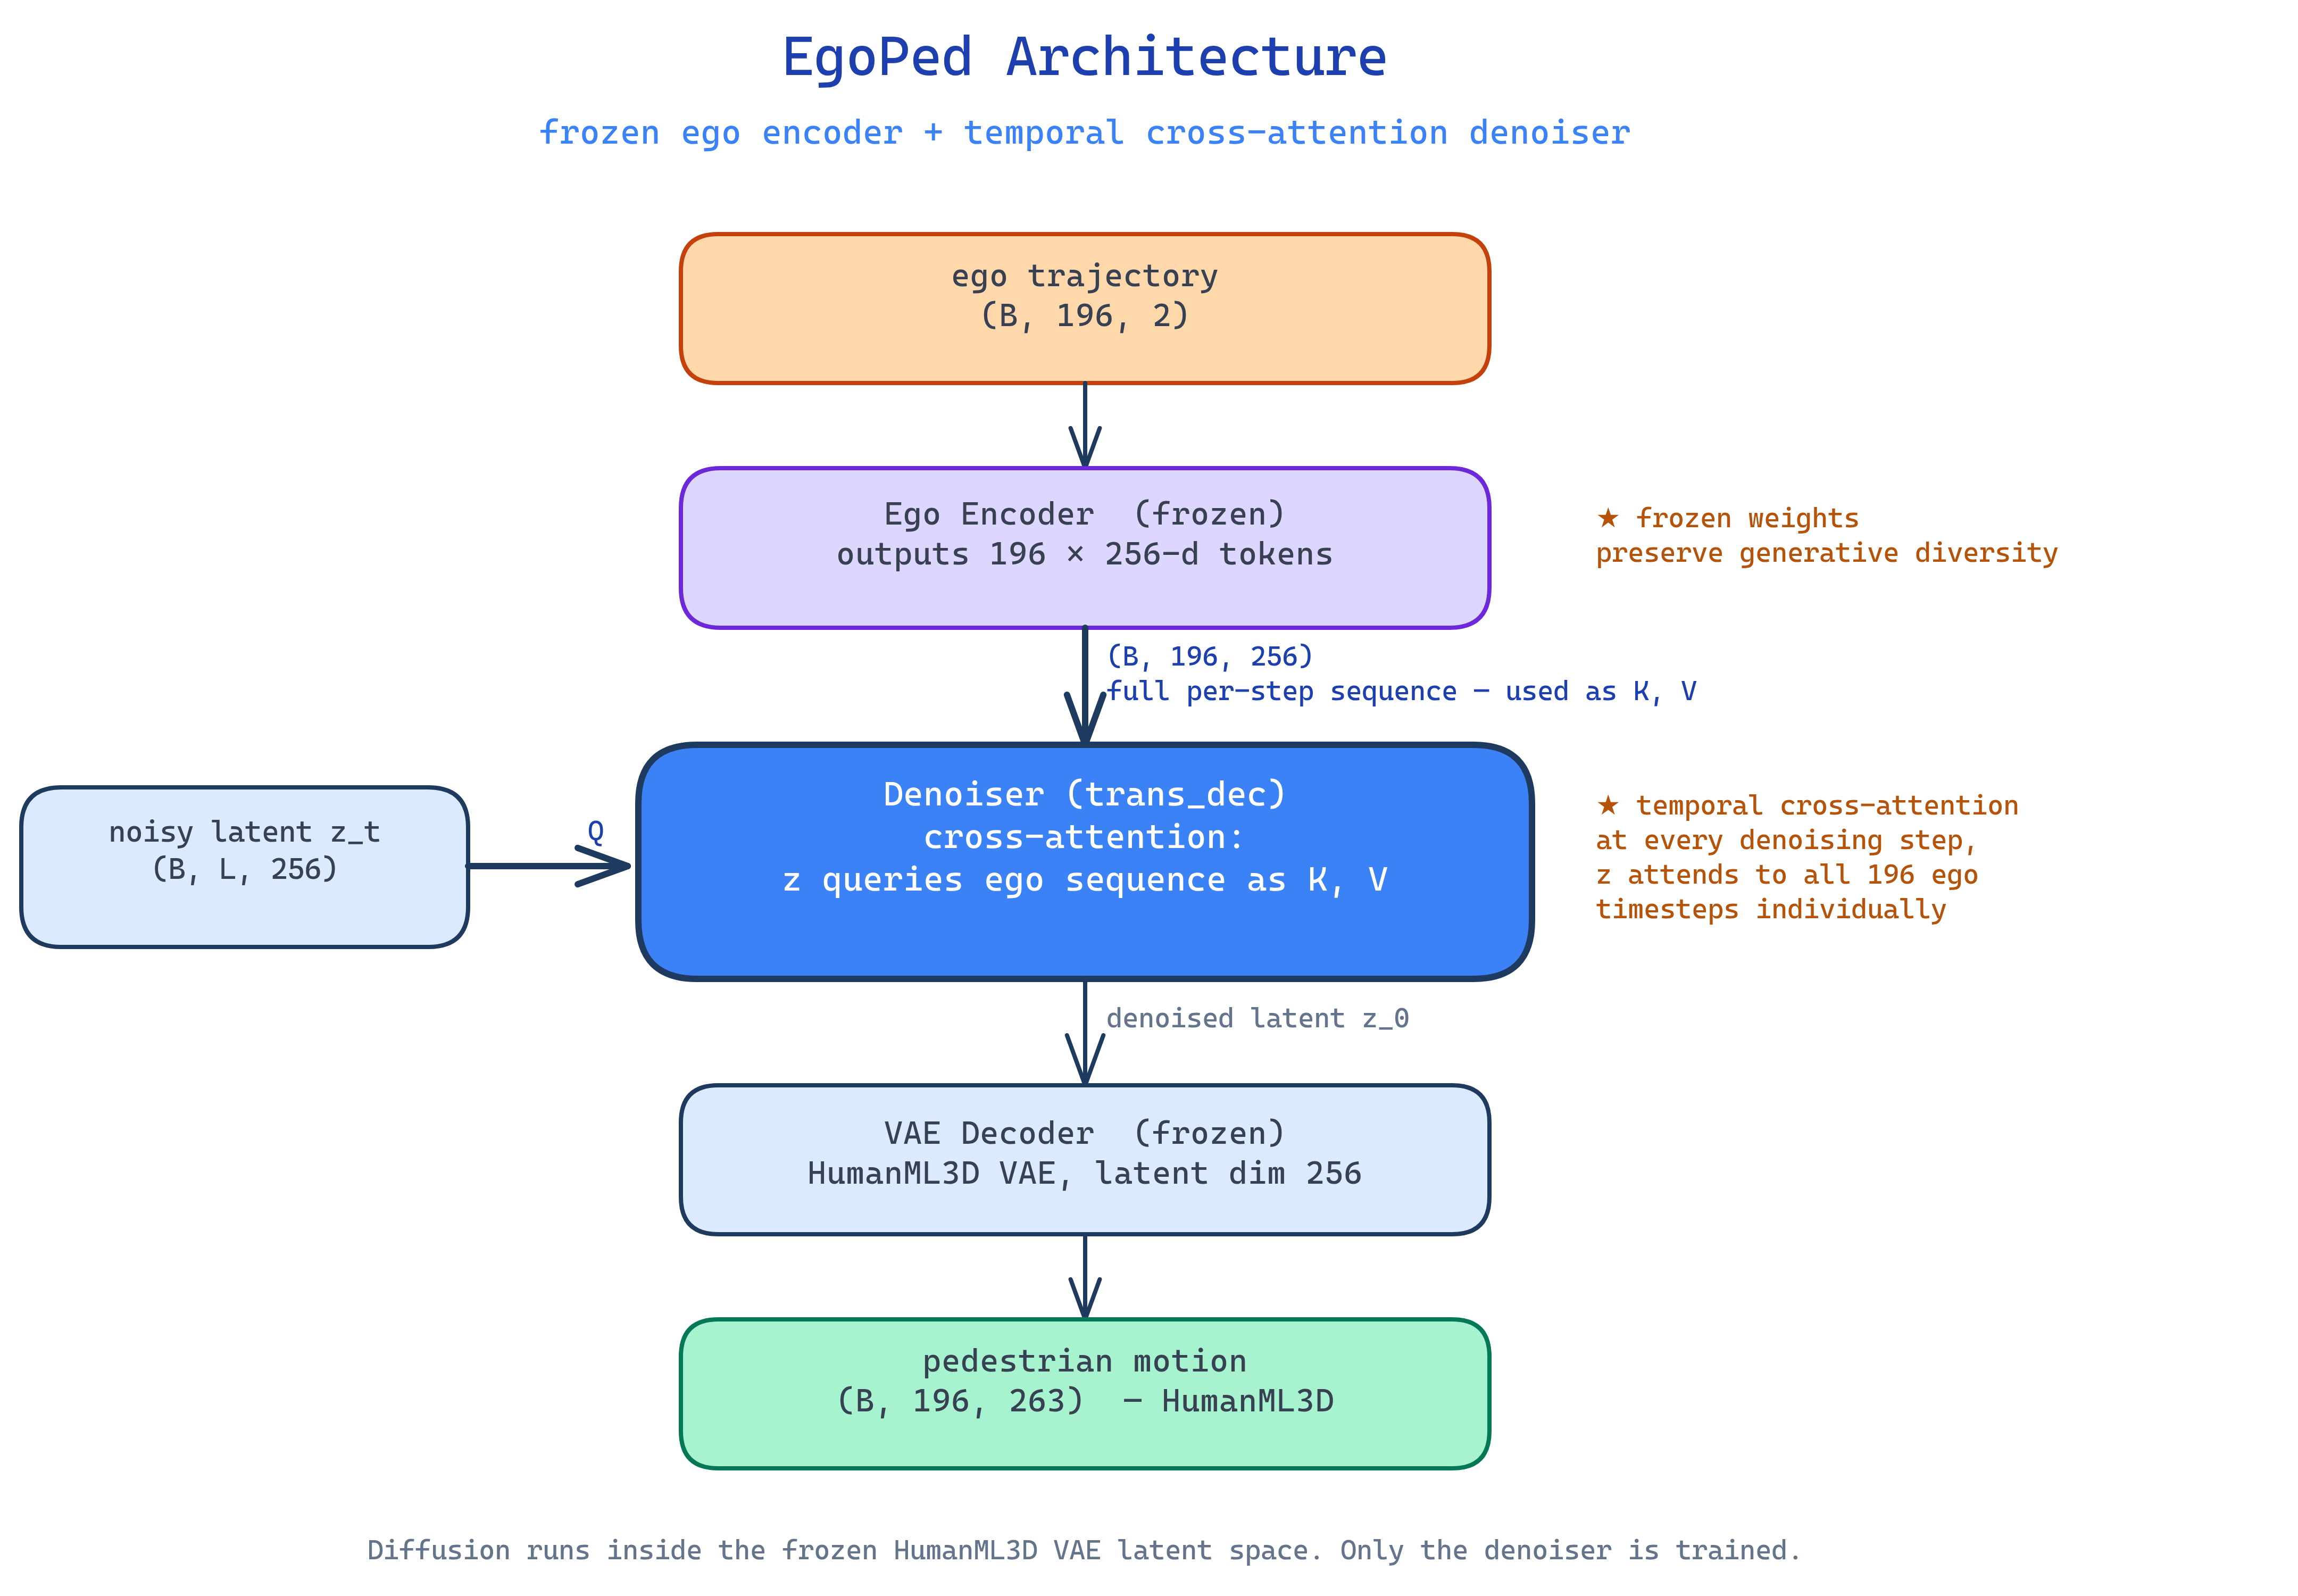
\includegraphics[width=0.92\linewidth]{figures/architecture.png}
  \caption{\method architecture. The ego trajectory is encoded by a \emph{frozen} transformer encoder into 196 per-timestep conditioning tokens. At every denoising step, the noisy latent $\mathbf{z}_t$ is concatenated with the full 196-token ego sequence (and the timestep embedding) and jointly processed by a self-attention transformer denoiser; the latent output tokens predict the noise. Diffusion runs in the latent space of a frozen HumanML3D VAE; only the denoiser is trained. Section~\ref{sec:xattn} ablates an alternative cross-attention denoiser.}
  \label{fig:architecture}
\end{figure*}

\subsection{Problem Formulation}

Given a vehicle ego trajectory $\mathbf{e} \in \mathbb{R}^{T \times 2}$ (2D position over $T=196$ timesteps), we aim to generate a plausible 3D pedestrian body motion $\mathbf{x} \in \mathbb{R}^{T \times 263}$ in the HumanML3D representation~\cite{guo2022humanml3d}.
The 263D representation encodes root velocity, root angular velocity, joint positions, velocities, and foot contact labels, fully parameterizing a SMPL-like body in motion.

We model the conditional distribution $p(\mathbf{x} \mid \mathbf{e})$ using a latent diffusion model that denoises within a pre-trained VAE's latent space.

\subsection{Motion VAE}

We use the MLD VAE~\cite{chen2023mld}, a Transformer encoder-decoder that compresses $T \times 263$ motion to a latent $\mathbf{z} \in \mathbb{R}^{L \times 256}$ with $L = 4$ latent tokens ($L$ is a hyperparameter; we find $L=4$ significantly outperforms $L=8$, see Section~\ref{sec:ablation}).
The VAE is pre-trained on the HumanML3D dataset and held fixed throughout diffusion training.

\subsection{Ego Encoder}

The ego trajectory $\mathbf{e} \in \mathbb{R}^{196 \times 2}$ is encoded by a lightweight transformer encoder:
\begin{equation}
  \mathbf{c} = \mathrm{EgoEncoder}(\mathbf{e}) \in \mathbb{R}^{196 \times 256}.
\end{equation}
The encoder consists of a linear projection from 2D to 256D, followed by sinusoidal positional encodings, and $N=4$ transformer encoder layers with 4 heads.
Unlike the pooled variant (Pooled), which applies mean-pooling to produce a single token $\mathbf{c} \in \mathbb{R}^{1 \times 256}$, our encoder preserves the full temporal sequence.

\paragraph{Ego encoder pretraining.}
Before diffusion training, the ego encoder is pretrained with a regression-based alignment objective that distills the paired motion's VAE latent into the ego encoding.
Specifically, we align the mean-pooled ego encoding $\bar{\mathbf{c}} = \mathrm{MeanPool}(\mathbf{c}) \in \mathbb{R}^{256}$ with the mean-pooled VAE posterior mean $\bar{\mathbf{z}} \in \mathbb{R}^{256}$ (computed from the paired motion) using a combined MSE and cosine objective:
\begin{equation}
  \mathcal{L}_{\mathrm{pretrain}} = \|\bar{\mathbf{c}} - \bar{\mathbf{z}}\|^2 + \lambda_{\cos}\bigl(1 - \cos(\bar{\mathbf{c}}, \bar{\mathbf{z}})\bigr),
\end{equation}
where the cosine term encourages directional alignment in addition to magnitude.
After pretraining, the encoder achieves validation MSE $\approx 1.92$, matching the pooled variant (which uses an additional 2-layer projection head without improvement), confirming that the projection head adds no alignment capacity.

\paragraph{Frozen encoder (key design choice).}
During diffusion training, the ego encoder parameters are \emph{frozen}.
This preserves the encoder's learned alignment while ensuring the generated motion distribution is not over-constrained to particular ego conditions.
We ablate this choice in Section~\ref{sec:ablation}.

The overall architecture is shown in Figure~\ref{fig:architecture}.

\subsection{Diffusion Denoiser}

We use the MLD denoiser as a self-attention transformer that operates over a single concatenated token sequence.
At each denoising step, the $L=4$ noisy latent tokens $\mathbf{z}_t$, the timestep embedding $\mathbf{t}_{\mathrm{emb}}$, and the full $T=196$-token ego conditioning sequence $\mathbf{c}$ are concatenated into one sequence of length $L + 1 + T = 201$ and processed by the transformer; the first $L$ output tokens are read out as the predicted noise:
\begin{equation}
  \hat{\boldsymbol{\epsilon}} = \boldsymbol{\epsilon}_\theta(\mathbf{z}_t, t, \mathbf{c}) = \mathrm{Transformer}\bigl([\mathbf{z}_t,\, \mathbf{t}_{\mathrm{emb}},\, \mathbf{c}]\bigr)_{1:L},
\end{equation}
where the transformer applies self-attention over the joint sequence and the sampler computes $\mathbf{z}_{t-1}$ from $\hat{\boldsymbol{\epsilon}}$.
Because every ego token participates in the same self-attention as the latent tokens, each denoising step has access to the full ego trajectory at per-timestep resolution: the denoiser can attend to specific moments in the ego trajectory (e.g., a braking event or sharp turn) rather than a global average.
This is the key distinction from the pooled baseline (Pooled), whose denoiser sees only a single mean-pooled ego token ($L+2$ tokens in total) and therefore has no temporal resolution over the ego trajectory.

The added cost over the pooled baseline is modest at this scale: self-attention over $201$ tokens versus $L+2$.
A natural alternative is a \emph{cross-attention} denoiser, in which the $L$ latent tokens act as queries and the ego sequence as keys/values, reducing the attention cost to $\mathcal{O}(L \times T)$ rather than $\mathcal{O}((L+T)^2)$.
We evaluate this variant in Section~\ref{sec:ablation} and find it performs \emph{comparably}, indicating that the benefit comes from exposing the denoiser to the full ego sequence, not from the specific attention mechanism used to inject it.

\subsection{Classifier-Free Guidance}

We train with classifier-free guidance~\cite{ho2022cfg}: for 10\% of training samples, the input ego trajectory is zeroed before encoding, so the encoder's response to the all-zero trajectory serves as the unconditional embedding (the same construction is used for the unconditional branch at inference).
At inference, the guided score is:
\begin{equation}
  \hat{\boldsymbol{\epsilon}}_t = \boldsymbol{\epsilon}_\theta(\mathbf{z}_t, \emptyset) + w \cdot \bigl(\boldsymbol{\epsilon}_\theta(\mathbf{z}_t, \mathbf{c}) - \boldsymbol{\epsilon}_\theta(\mathbf{z}_t, \emptyset)\bigr),
\end{equation}
with guidance scale $w$.
We find $w = 10$ optimal for \method (Section~\ref{sec:experiments}).

\subsection{Training Objective}

The denoiser is trained with the standard DDPM noise-prediction objective:
\begin{equation}
  \mathcal{L} = \mathbb{E}_{\mathbf{z}_0, \boldsymbol{\epsilon}, t} \bigl[\|\boldsymbol{\epsilon} - \boldsymbol{\epsilon}_\theta(\mathbf{z}_t, t, \mathbf{c})\|^2\bigr].
\end{equation}
We use DDIM~\cite{song2021ddim} for fast inference with 50 denoising steps.

%----------------------------------------------------------------------
\section{Experiments}
\label{sec:experiments}
%----------------------------------------------------------------------

\subsection{Dataset}

As there are no datasets available for the problem investigated in this work, we generated a dataset for ego-conditioned motion generation from two complementary sources: existing large-scale autonomous driving datasets (nuScenes~\cite{caesar2020nuscenes}, Waymo~\cite{sun2020waymo}), which supply scale and behavioral diversity, and a small, deliberately \emph{staged} set of high-interaction scenes recorded with our sensor-equipped research vehicle AVA, which targets the close-range vehicle--pedestrian encounters that are rare in the public datasets. The vehicle is equipped with seven 128-layer LiDARs and eight RGB cameras for full 360° sensor coverage around the vehicle. To obtain scenes with meaningful interaction between the vehicle and a pedestrian, we staged \TODO{NUMBER} highly interactive scenarios. The recorded data is brought into nuScenes format and objects in the scene are annotated with 3D bounding boxes and orientation labels using MS3D \cite{tsai2024ms3d++, tsai2023ms3d}.

With the data in nuScenes format fully annotated, we extract 3D human poses in SMPL~\cite{SMPL:2015} format using an adapted version of OmniRe~\cite{chen2025omnire} from all three data sources: AVA, nuScenes, and Waymo Open Dataset. We estimate poses for every pedestrian instance from all available camera images, using the projected 3D bounding box to localize the person in each view. Per-instance pose estimates from different cameras are then stitched into a single continuous sequence using the extrinsic calibration of the camera rigs. Finally, the SMPL pose sequences are converted to the 263D HumanML3D motion representation~\cite{guo2022humanml3d}, which retargets every sequence onto a single canonical skeleton; body shape is therefore not represented in our data (Sec.~\ref{sec:posequality}). In addition to the pedestrian pose sequences, we extract the synchronized ego-vehicle trajectory from each scene's odometry.
A single automated pipeline processes every (scene, pedestrian) pair end-to-end: it loads the annotated nuScenes-format scene, extracts and stitches the per-instance SMPL body sequence, resamples both the body motion and the ego odometry to a common $20$~fps grid, and expresses both streams in a \emph{pedestrian-centric} coordinate frame (translation- and yaw-normalized to the pedestrian) so that conditioning is invariant to the absolute world pose of the scene.
Each resulting sample is stored as a self-contained record containing the pedestrian's 22 body-joint positions $(\texttt{ped\_in\_ped\_frame} \in \mathbb{R}^{T\times 22\times 3})$, the ego trajectory in the same frame $(\texttt{ego\_in\_ped\_frame} \in \mathbb{R}^{T\times 3})$, and the derived 263D HumanML3D motion vector $(\texttt{vectors\_263} \in \mathbb{R}^{T\times 263})$, where the native sequence length $T$ varies per scene and is windowed to $196$ frames at training time (see the interaction-aware cropping procedure below).

Using all three data sources we obtain \textbf{11{,}954} paired ego--pedestrian motion samples in total, split by scene into 9{,}540 training and 2{,}414 validation samples with no scene overlap between the two splits. Per-source counts are given in Table~\ref{tab:dataset}. Waymo and nuScenes dominate the sample count, while the AVA recordings contribute a small but deliberately high-interaction subset of staged vehicle--pedestrian encounters.

\begin{table}[t]
  \centering
  \caption{Dataset composition. Each sample is a paired sequence of ego odometry ($196\times2$) and pedestrian body motion ($196\times263$), extracted from AVA, nuScenes, and Waymo. Train/validation splits are disjoint at the scene level; the validation split is the evaluation set used for all reported metrics.}
  \label{tab:dataset}
  \vspace{4pt}
  \small
  \setlength{\tabcolsep}{8pt}
  \begin{tabular}{lccc}
    \toprule
    Source & Train & Validation & Total \\
    \midrule
    AVA (ours)          & 27    & 7     & 34 \\
    nuScenes            & 3{,}637 & 943   & 4{,}580 \\
    Waymo Open Dataset  & 5{,}876 & 1{,}464 & 7{,}340 \\
    \midrule
    Total               & 9{,}540 & 2{,}414 & 11{,}954 \\
    \bottomrule
  \end{tabular}
\end{table}

Each sample is a paired sequence of ego odometry $\mathbf{e} \in \mathbb{R}^{196 \times 2}$ and pedestrian body motion $\mathbf{x} \in \mathbb{R}^{196 \times 263}$, both expressed in the pedestrian-centric frame.

\paragraph{Interaction scoring.}
Rather than hard-filtering samples, we assign each scenario a scalar \emph{interaction score} that quantifies how strongly the pedestrian and ego vehicle interact, and use it both to bias training-time sampling and to guide cropping.
Let $\mathbf{r}_t, \mathbf{g}_t \in \mathbb{R}^2$ denote the ground-plane (XZ) positions of the pedestrian pelvis and the ego vehicle at frame $t$. The score combines three factors:
\begin{equation}
  s = s_{\text{travel}} \cdot s_{\text{prox}} \cdot s_{\text{bearing}},
\end{equation}
with the three factors
\begin{align}
  s_{\text{travel}}  &= \sum_{t} \lVert \mathbf{r}_{t+1} - \mathbf{r}_t \rVert_2, \\
  s_{\text{prox}}    &= \frac{1}{T}\sum_t \mathbb{1}\!\left[\lVert \mathbf{g}_t - \mathbf{r}_t \rVert_2 < 5\,\text{m}\right], \\
  s_{\text{bearing}} &= 1 + \frac{1}{180^\circ}\sum_t \lvert \Delta\phi_t \rvert,
\end{align}
measuring pedestrian travel, the fraction of frames spent in proximity, and the swept relative bearing.
Here $\mathbb{1}[\cdot]$ denotes the indicator function, $\phi_t = \operatorname{atan2}(\mathbf{r}_t - \mathbf{g}_t)$ is the pedestrian's bearing relative to the ego vehicle, and $\Delta\phi_t$ is the (wrap-corrected) inter-frame change in bearing.
Intuitively, a scenario scores highly when the pedestrian moves substantially, spends many frames within 5\,m of the vehicle, and sweeps a large relative bearing (\eg crossing in front of the vehicle).

\paragraph{Interaction-weighted sampling.}
The pipeline supports drawing training samples with a \texttt{WeightedRandomSampler} whose weights are the interaction scores $s$ (floored at $0.01$ so low-interaction scenarios are still occasionally seen, then normalized to sum to the dataset size), concentrating gradient updates on the ego-relevant portion of the data distribution without discarding any samples. The VAE, the pooled baseline (Pooled), and our best system (\method-IA) train with this weighting; the \method reference model trains with uniform sampling, and we disentangle the two effects with a full 2$\times$2 ablation in Section~\ref{sec:pipeline2x2}. Evaluation always uses uniform (unweighted) sampling.

\paragraph{Interaction-aware cropping.}
To bound the generation problem to a fixed horizon, we crop each scenario to $T=196$ timesteps ($\approx$40\% of sequences are longer). The pipeline supports centring the crop on the \emph{closest-approach frame} $t^\star = \arg\min_t \lVert \mathbf{g}_t - \mathbf{r}_t \rVert_2$, with uniform jitter of $\pm 25\%$ of the window length so the moment of closest approach is not memorized at a fixed position (the window is clamped to lie within the sequence); the alternative is a uniformly random window. The VAE, Pooled, and \method-IA use interaction-centred crops; the \method reference model uses random windows (ablated in Section~\ref{sec:pipeline2x2}). In both modes, ego and motion streams are cropped with a shared index so they stay temporally aligned, and scenarios shorter than 196 frames are zero-padded at the end with their true length recorded for masking.

\subsection{Pseudo-Ground-Truth Pose Quality}
\label{sec:posequality}
Our pose labels are OmniRe estimates rather than measured 3D ground truth, and no reference source (mocap or manual annotation) exists for these scenes. We therefore audit what can be checked \emph{without} a reference --- internal physical consistency --- over all 14{,}172 extracted sequence files (13{,}958 of them long enough to score); the audit script is released with the code. This population is deliberately the full extraction, a superset of the 11{,}954 samples the benchmark splits retain (Table~\ref{tab:dataset}), so the audit characterizes the label pipeline rather than only the sequences we train on. Table~\ref{tab:posequality} reports the result, and it materially qualifies how our metrics should be read.

Three things stand out. First, \textbf{body shape was never estimated}: every sequence in all three sources shares one skeleton to within $10^{-5}$ relative bone length, so the corpus contains a single canonical body rather than per-person shapes. This also means bone-length and left/right-symmetry checks carry no quality signal here, since rigidity is imposed by the representation rather than recovered from images. Second, \textbf{the feet do not plant}. During locomotion at least one foot should be stationary in world coordinates; taking the slowest of the four foot joints per frame and dividing by root speed gives a median ratio of $0.97$, where $0$ denotes clean footfalls and $1$ a body sliding as a rigid unit, and $94.6\%$ of moving sequences never hold a foot still for more than $5\%$ of their frames. This check is internal and has no domain confound. Third, \textbf{articulation is damped} relative to real mocap: against HumanML3D's own per-dimension statistics, root translation is \emph{more} variable than mocap ($1.29\times$) while root-relative joint positions, root height and turning are far less ($0.44\times$, $0.26\times$, $0.37\times$). Part of that gap is content rather than quality --- HumanML3D spans every kind of motion and ours is people walking near roads --- so we read it as corroborating the foot-skate result rather than as an independent measurement.

\paragraph{Where the sliding lives.} Because the artifact is in the labels, it is worth asking whether it is also in the model, and whether a training-side fix could remove it. We apply the identical foot-skate measure at three points of the pipeline on the same held-out conditions (Table~\ref{tab:skate}). The labels slide at 0.96; a VAE round-trip of those labels, which involves no diffusion model at all, already slides at 0.94; and samples from the trained models slide at 0.93--0.94. Two things follow. Our models neither amplify nor repair the artifact --- they are faithful fits to a target that slides, which is the expected behaviour of a well-trained generative model and not an independent failure. And because the frozen VAE reproduces the sliding on its own, the artifact is embedded in the latent space that every denoiser in this paper decodes through, so a contact or foot-skate penalty applied to the denoiser would be optimizing against its own decoder. Removing the sliding therefore requires correcting the labels and retraining the VAE, which changes the target distribution and invalidates every FID value reported here, so we do not attempt it for this paper. We did run a feasibility pilot, because the more damaging possibility is that the latent bottleneck itself cannot represent planted feet. Anchoring footfalls to the measured root path (preserving the root and upper body, re-solving the legs by inverse kinematics) removes the sliding from the labels, and on 1{,}418 such sequences the original VAE reconstructs them at a skate ratio of 0.75 --- it pulls clean input back toward sliding --- whereas a VAE fine-tuned for 400 epochs on the corrected labels reconstructs at 0.15. The representation is therefore not the obstacle, and relabelling is a viable if expensive direction. We note also that any correction that preserves the tracked root --- the component this audit finds sound --- must re-synthesize the legs, replacing estimated poses with procedurally generated gait, which is a different trade rather than a strictly better ground truth.

\begin{table}[t]
  \centering
  \caption{Reference-free audit of the pseudo-ground-truth poses (13{,}958 sequences; 10{,}900 contain locomotion). Upper block: internal physical consistency, no external reference and no domain confound. Lower block: ratio of our per-dimension standard deviation to HumanML3D's real-mocap statistics, by block of the 263-D representation; values below 1 indicate less variability than mocap, though part of that gap reflects the narrower motion content of driving scenes.}
  \label{tab:posequality}
  \vspace{4pt}
  \footnotesize
  \begin{tabular}{lc}
    \toprule
    Internal consistency check & Result \\
    \midrule
    Distinct skeletons among all sequences & 1 \\
    Max.\ relative bone-length deviation & $6.3\times10^{-6}$ \\
    Foot-skate ratio, median (0 = plant, 1 = slide) & 0.97 \\
    \quad AVA / nuScenes / Waymo & 0.73 / 0.99 / 0.95 \\
    Never plant a foot ($>$5\% of moving frames) & 94.6\% \\
    Near-static legs (ankle swing $<$ 5\,cm) & 14.1\% \\
    Ground penetration $>$ 5\,cm & 1.2\% \\
    \midrule
    Variability vs.\ mocap (ours / HumanML3D std) & Ratio \\
    \midrule
    Root linear velocity & 1.29 \\
    Joint rotations & 0.68 \\
    Root-relative joint positions & 0.44 \\
    Root rotational velocity & 0.37 \\
    Root height & 0.26 \\
    \bottomrule
  \end{tabular}
\end{table}

The picture is a lightly articulated canonical body translating along a well-tracked trajectory. That asymmetry maps cleanly onto our conclusions. The evidence that conditioning is \emph{used} --- root ADE/FDE (Sec.~\ref{sec:adefde}) and the stop/walk probe (Sec.~\ref{sec:behavior}) --- is computed from the root trajectory, the component this audit finds trustworthy, so those conclusions are unaffected. FID is the exposed quantity: it scores body pose against this same damped target, which makes the marginal easier to fit than the visual richness of real pedestrians would suggest and helps explain why an ego-blind prior can reach FID 1.43 (Table~\ref{tab:trivial}). Absolute FID values here should be read as within-benchmark comparisons only, never as a claim about pose realism.

\begin{table}[t]
  \centering
  \caption{Foot-skate ratio measured at three points of the pipeline (held-out split, same metric as Table~\ref{tab:posequality}; 0 = clean footfalls, 1 = the body sliding as a rigid unit). The VAE round-trip involves no diffusion model, so the sliding is already present in the latent representation; the generative models inherit it without amplifying it.}
  \label{tab:skate}
  \vspace{4pt}
  \footnotesize
  \begin{tabular}{lcc}
    \toprule
    Pipeline stage & Skate & Planted (\%) \\
    \midrule
    Pseudo-ground-truth labels & 0.96 & 0.6 \\
    VAE round-trip (encode--decode) & 0.94 & 0.0 \\
    Generated, \method & 0.94 & 0.0 \\
    Generated, \method-IA & 0.93 & 0.0 \\
    Generated, unconditional prior & 0.84 & 0.6 \\
    \bottomrule
  \end{tabular}
\end{table}

\subsection{Evaluation Protocol}
\label{sec:eval}

We report four metrics, following the HumanML3D evaluation protocol~\cite{guo2022humanml3d}:

\begin{itemize}
  \item \textbf{FID} (Fréchet Inception Distance): computes the feature-space distance between the generated and real motion distributions, using the pretrained \texttt{t2m\_moveencoder} (stride-2 Conv1D) and \texttt{t2m\_motionencoder} (BiGRU) from~\cite{guo2022humanml3d}. Lower is better.
  \item \textbf{R-Precision@1}: top-1 retrieval accuracy of the ego condition from batches of 32 candidates (1 positive + 31 negatives), using cosine similarity between the mean-pooled VAE latent (from generated motion) and the ego encoder output. Higher is better.
  \item \textbf{MultiModality (MM)}: average pairwise L2 distance between 10 generated samples for the same ego condition, measuring diversity per condition. Higher indicates more diverse generation per condition, but is only meaningful at comparable conditioning fidelity — an unconditional model maximizes MM trivially (cf.\ Table~\ref{tab:trivial}) — so MM should be read jointly with R-Precision.
  \item \textbf{Diversity}: average pairwise L2 distance in feature space across all generated samples, measuring population-level diversity. Values \emph{closer to the ground-truth diversity} (5.496 on our evaluation set) are better.
\end{itemize}


All reported values are the mean over \textbf{3 independent replications} with 95\% confidence intervals.
Unless stated otherwise, metrics are computed on the full validation split (2{,}414 samples), which is also used for checkpoint selection, under a \emph{unified evaluation pipeline}: identical eval-time data processing (uniform sampling, random 196-frame windows) for every system, regardless of its training-time data pipeline. Earlier internal evaluations mixed per-model eval pipelines; all headline comparisons in this paper are unified.
To control for selection bias, we additionally construct a \emph{held-out test split}: the validation scenes are partitioned into two scene-disjoint halves, one reserved purely for held-out reporting (1{,}190 samples from 521 scenes, never used for any model or checkpoint selection of our main system).
Our best system reproduces its headline result on this held-out split (FID $= 3.34 \pm 0.19$ vs.\ $3.39 \pm 0.18$ on the full validation split), confirming the result is not an artifact of evaluating on the selection set; the conditioning-mechanism ablation (Section~\ref{sec:xattn}) is reported on this split.
Note that FID and Diversity use a fixed, pretrained evaluator shared by all systems, so they are directly comparable across architectures.
R-Precision, in contrast, retrieves with each model's \emph{own} ego encoder embedding; cross-architecture R@1 comparisons (\eg pooled vs.\ full-sequence encoders) should therefore be read as indicative rather than exact, as the retrieval space itself differs.

\subsection{Implementation Details}
\label{app:impl}

\paragraph{Ego encoder.}
4-layer transformer encoder, 4 attention heads, 256D hidden dimension (1024D feed-forward), sinusoidal positional encoding for $T=196$ timesteps.
Input: 2D ego position sequence, projected linearly to 256D.
No projection head (we verified the 2-layer MLP projection head does not improve val MSE: 1.919 vs.\ 1.920).
Pretraining: AdamW (lr $= 1\times10^{-4}$, weight decay $10^{-4}$), 200 epochs, batch size 64, linear warmup followed by cosine annealing, gradient clipping at max-norm 1.0.

\paragraph{Diffusion model.}
MLD denoiser in the self-attention configuration (attending over the concatenated latent, timestep, and ego tokens): 9 layers, 4 attention heads, 256D token dimension, 1024D feed-forward, latent sequence length $L=4$. The cross-attention variant of Section~\ref{sec:xattn} uses the same hyperparameters in a cross-attention configuration (latent tokens as queries, ego sequence as keys/values).
Diffusion: 1000 DDPM training steps (scaled-linear $\beta$ schedule), DDIM inference (50 steps, $\eta=0$).
CFG dropout rate: 10\%.
Optimizer: AdamW, lr $= 1\times10^{-4}$ (constant), 5000 total epochs.
Batch size: 128.
Training hardware: NVIDIA H100 (80 GB) on an academic HPC cluster; training runs in segments of up to 24h wall time.

\paragraph{Checkpoint selection.}
We select checkpoints based on validation FID (not training loss).
For \method, epoch 3399 is best; we confirm this with the full training trajectory and definitive 3-replication evaluation.
For Pooled, epoch 4399 is best despite continued training to epoch 5000.

\paragraph{Evaluation.}
All evaluations use 3 independent generation passes,
300 samples for Diversity, and 100 conditions $\times$ 10 repeats for MultiModality.
Each replication regenerates the full test set with fresh sampling noise; the diffusion sampler is stochastic across replications while the data pipeline and evaluator are fixed (training uses seed 1234).
Confidence intervals are reported as $\pm$~CI (half-width of the 95\% interval across replications).

\subsection{Baselines}

\begin{itemize}
  \item \textbf{Pooled (our baseline)}: pooled ego encoder (transformer + mean-pool $\to$ single 256D token), self-attention denoiser (concatenated self-attention over $[\mathbf{z}, \mathbf{c}_\mathrm{pool}, \mathbf{t}]$). Best at epoch 4399, CFG~=~5.
  \item \textbf{Latent-8}: Same as Pooled but with latent dimension $L=8$ (larger VAE). Best at epoch 4399, CFG~=~5.
\end{itemize}

We additionally report four non-learned or reference baselines (Table~\ref{tab:trivial}) that bound the metric space.
\textbf{Unconditional MLD} runs our \method model (epoch 3399) with every ego trajectory zeroed; because CFG training dropout uses the same zeroed-trajectory construction, both guidance branches receive identical embeddings and guidance cancels exactly, so guidance cancels and the model falls back on whatever it learned to produce without the ego. We report it because the literature uses this construction, not because it is a well-trained prior --- the separately trained models below show it is not. A \emph{separately trained} unconditional model (identical recipe, ego dropped at every training step, 5,000 epochs, evaluated through the same ego-zeroing at guidance scale 1) reaches FID 3.24 $\pm$ 0.13 --- statistically indistinguishable from the full-sequence model (3.39 $\pm$ 0.18). FID therefore does not by itself credit ego conditioning: the ego-zeroed branch of a conditional model is merely a weak unconditional generator, and a well-trained prior matches the conditional model's \emph{marginal}. Repeating the control on the interaction-sampling data recipe is more striking still: an unconditional model trained that way reaches FID 1.43 $\pm$ 0.18 --- the best marginal of any model in this paper, better than \method-IA (2.88 $\pm$ 0.08) with non-overlapping intervals --- while being demonstrably ego-blind (ADE 3.00, behavioural separation 0.02, R@1 at chance). Interaction sampling is therefore largely a \emph{marginal-quality} intervention: it improves the prior (3.24 $\to$ 1.43) more than it improves the conditional model (3.39 $\to$ 2.88), so \method-IA's FID advantage does not survive comparison against its own prior. Evidence that the conditioning is used comes from the evaluator-independent trajectory metrics (Sec.~\ref{sec:adefde}) and the behavioral probe (Sec.~\ref{sec:behavior}), which a model without ego access cannot match.
\textbf{Retrieval} returns, for each test ego trajectory, the training motion whose ego trajectory is the nearest neighbour (32-point resampled L2).
\textbf{VAE interpolation} decodes a random latent interpolation of two training motions.
\textbf{Trajectory$+$kinematic} replaces all body features with the training mean, keeping either the ground-truth root velocity (\emph{oracle}) or nothing (\emph{mean}), simulating a trajectory-prediction-then-fitting pipeline with no learned body model.
We further add two \emph{learned} baselines trained on the identical data recipe with the same frozen ego encoder.
\textbf{Ego$\to$motion regressor}: a deterministic sequence-to-sequence transformer regressing the 263-D features with masked MSE — the conditional-mean predictor.
\textbf{Raw-space diffusion (MDM-style)}: our diffusion model operated directly in the 263-D feature space without the latent VAE (a same-capacity raw-space variant in the spirit of MDM~\cite{tevet2023mdm}, not a faithful reproduction); its best checkpoint plateaus early and never approaches latent-space quality, justifying the latent backbone.
\textbf{Pretrained text-to-motion MLD}: the released HumanML3D MLD checkpoint~\cite{chen2023mld} generating from a text prompt instead of ego trajectory, evaluated on our held-out conditions. Because it is trained on a different corpus (mocap-quality everyday motion) its gap to our in-domain models conflates domain shift with the conditioning question; we therefore read it as evidence that off-the-shelf text-to-motion does not transfer to driving-scene pedestrians, rather than as a statement about text versus ego conditioning per se.

\paragraph{Information ladder: how much conditioning information is needed?}
To separate \emph{that} a condition helps from \emph{how much} information it must carry, we train the same architecture with conditioning signals of increasing information content (Table~\ref{tab:ladder}) and evaluate all of them with the unified pipeline. Captions are synthesized deterministically from kinematics for all 14,172 sequences, and the information content is the entropy of the resulting template distribution. The \emph{vehicle-only} vocabulary describes only what the ego-trajectory model sees (approach/pass/wait, side, proximity, ego speed and turning, timing of closest approach). The \emph{oracle} vocabulary additionally verbalizes the pedestrian's own ground-truth behaviour (gait, turning, stopping); it is therefore an upper bound, not a competitor. Text models use 10\% caption dropout and CLIP text features, and are evaluated at the same CFG scale as the trajectory models (a sweep over \{1, 2.5, 5, 10\} is monotone for the oracle model: 6.43, 5.71, 4.14, 2.82). The vehicle-only model is evaluated on a $3$-epoch$\times$$4$-CFG grid (epochs 99, 3399, 4999; FID ranges from 5.12 at epoch 99 with CFG 5 to 6.67); its epoch-matched checkpoint reaches FID 5.91, ADE 2.52 and behavioural separation 0.21 --- roughly two thirds of the trajectory model's per-condition gains over the unconditional prior (ADE $2.99\to2.32$, separation $0.04\to0.33$) at a much worse marginal, so a coarse verbal description of the vehicle carries real but incomplete ego information, and the continuous trajectory supplies the rest on both axes. Its FID-best checkpoint (epoch 99, FID 5.12) is behaviourally ego-blind (separation 0.05), reproducing within a single model the dissociation between FID and conditioning.
\begin{table*}[t]
  \centering
  \caption{Reference baselines bounding the metric space (val split; same evaluator, normalization, and split lists as Table~\ref{tab:main}). All rows are mean $\pm$ 95\% CI over 3 replications (the unconditional row resamples the diffusion model; the non-learned rows are reseeded end-to-end). Retrieval attains near-zero FID by copying real motions but is non-generative; trajectory$+$kinematic shows that following the root trajectory with a static body is catastrophic. The 5.18 row is \emph{not} a prior: it is the under-trained null branch of a conditional model, and separately trained unconditional models reach 3.24 on the standard recipe and 1.43 with interaction sampling. FID differences across these rows therefore order marginal fit, not the use of the ego; see Sec.~\ref{sec:adefde} and Sec.~\ref{sec:behavior}.}
  \label{tab:trivial}
  \vspace{4pt}
  \small
  \setlength{\tabcolsep}{5pt}
  \begin{tabular}{lccc}
    \toprule
    Method & FID $\downarrow$ & Diversity & R@1 $\uparrow$ \\
    \midrule
    Retrieval (NN ego)$^\ast$        & 0.062 {\scriptsize $\pm$0.004} & 5.34 & -- \\
    Trajectory+kinematic (mean)      & 49.60 {\scriptsize $\pm$0.087} & 0.46 & -- \\
    Trajectory+kinematic (oracle)    & 47.67 {\scriptsize $\pm$0.085} & 0.72 & -- \\
    Pretrained text-to-motion MLD~\cite{chen2023mld}$^\S$ & 14.07 & 3.12 & --$^\ddagger$ \\
    Ego$\to$motion regressor (learned, deterministic) & 35.47 & 3.47 & -- \\
    Raw-space diffusion (learned, MDM-style)          & 26.43 {\scriptsize $\pm$0.098} & 3.55 & --$^\ddagger$ \\
    VAE latent interpolation         & 7.91 {\scriptsize $\pm$0.033}  & 5.82 & -- \\
    Unconditional \method (ego zeroed) & 5.18 {\scriptsize $\pm$0.209} & 5.96 & 0.031$^\dagger$ \\
    Unconditional \method (trained, $p_\mathrm{drop}{=}1$)$^\P$ & 3.24 {\scriptsize $\pm$0.130} & 5.91 & 0.031$^\dagger$ \\
    \quad + interaction sampling$^\P$ & 1.43 {\scriptsize $\pm$0.183} & 5.76 & 0.031$^\dagger$ \\
    \midrule
    Pooled                      & 5.620  & 5.82 & 0.665 \\
    \method                     & 3.392 & 5.79 & 0.548 \\
    \method-IA (ours)                & \textbf{2.880} & 5.67 & 0.323 \\
    \bottomrule
  \end{tabular}
  \\[2pt]
  {\footnotesize $^\ast$Non-generative upper bound: copies real training motions, so low FID reflects memorization rather than conditioned synthesis. $^\dagger$Exactly chance level ($1/32 = 0.031$), confirming the R-Precision protocol: without ego information, retrieval is random. $^\ddagger$R-Precision is undefined for these models (no shared embedding space with the ego encoder). $^\P$Trained with $p_\mathrm{drop}=1$ (never sees the ego) and evaluated through the same ego-zeroing path as the row above. Training-time validation feeds real ego to these models and is not a valid selector, so we evaluate three late checkpoints (epochs 3999/4499/4999) offline and report the best: epoch 4999 for the standard recipe (the three span 3.24--4.90) and epoch 4499 for the interaction-sampling recipe (span 1.43--2.67; even its worst checkpoint matches \method-IA). $^\S$Official HumanML3D checkpoint driven by a fixed text prompt; we report the \emph{best} of three prompts (a naive scene description, a HumanML3D-idiomatic phrase, and per-sample oracle captions derived from ground-truth motion), which spanned FID 14.07--24.84. Its output is converted from HumanML3D to our normalization before scoring with the shared evaluator.}
\end{table*}

\begin{table*}[t]
  \centering
  \caption{Information ladder (val split, unified pipeline, 3 replications; CFG 10 for all conditional models, CFG 1 for the unconditional one). FID orders the \emph{marginals}, not the conditioning: a well-trained unconditional model matches the trajectory model, and an oracle that is told the pedestrian's behaviour matches \method-IA. Whether a condition is actually \emph{used} is measured in Secs.~\ref{sec:adefde} and \ref{sec:behavior}. ADE (m) and behavioural separation (held-out split, $K{=}5$) show which signals are actually \emph{used}: the trained prior is ego-blind despite matching \method's FID, the oracle is told the answer, and interaction sampling improves the marginal but not the per-condition fidelity (bold: best non-oracle model). The vehicle-only row is the epoch-matched checkpoint; its FID-best checkpoint (5.12) does not use the condition. The dissociation is sharpest off the ladder: an unconditional model trained with \method-IA's own interaction-sampling recipe reaches FID 1.43, better than every conditional model here, at ADE 3.00 and separation 0.02 (Table~\ref{tab:trivial}).}
  \label{tab:ladder}
  \vspace{2pt}\small
  \begin{tabular}{lccccc}
    \toprule
    Conditioning signal & Information & FID $\downarrow$ & ADE $\downarrow$ & Separation $\uparrow$ & Diversity \\
    \midrule
    None (trained unconditional, $p_\mathrm{drop}{=}1$) & 0 bits & 3.24 {\scriptsize $\pm$0.130} & 3.01 & 0.05 & 5.91 \\
    Vehicle-only text (epoch-matched, 3399) & 5.17 bits & 5.91 {\scriptsize $\pm$0.055} & 2.48 & 0.21 & 5.67 \\
    Oracle text (+ ground-truth pedestrian behaviour) & 6.09 bits & 2.82 {\scriptsize $\pm$0.027} & 1.88 & 0.94 & 6.20 \\
    Ego trajectory (\method) & continuous, $196\times2$ & 3.39 {\scriptsize $\pm$0.179} & \textbf{2.36} & \textbf{0.33} & 5.79 \\
    Ego trajectory + interaction sampling (\method-IA) & continuous, $196\times2$ & \textbf{2.88} {\scriptsize $\pm$0.084} & 2.66 & 0.16 & 5.67 \\
    \bottomrule
  \end{tabular}

\end{table*}

\subsection{Main Results}
\label{sec:main}

Table~\ref{tab:main} shows the definitive evaluation results.
\method achieves FID $= 3.392 \pm 0.179$ at epoch 3399 and CFG $= 10$, a \textbf{40\% improvement} over the pooled baseline under the unified evaluation pipeline (FID $= 5.620 \pm 0.117$ at CFG $= 5$), and \method-IA improves this further to $2.880 \pm 0.084$.
The improvement is significant: the confidence intervals are non-overlapping (\method CI: $[3.213, 3.571]$; Pooled CI: $[5.503, 5.737]$).

\begin{table*}[t]
  \centering
  \caption{Main evaluation results under a \emph{unified} evaluation pipeline (identical eval-time data processing for all systems; each method at its own optimal CFG, sweep in Table~\ref{tab:cfg}). All values are mean $\pm$ 95\% CI over 3 replications. Best values in \textbf{bold}; for Diversity, values closer to the ground-truth reference are better. \method-IA additionally uses interaction-aware training-data sampling (Section~\ref{sec:pipeline2x2}); its FID replicates across two training seeds (2.880 and 2.671), whereas \method's seed sensitivity is much larger --- both are quantified in Section~\ref{sec:seeds}.}
  \label{tab:main}
  \vspace{4pt}
  \small
  \setlength{\tabcolsep}{4pt}
  \begin{tabular}{lcccccc}
    \toprule
    Method & Epoch & CFG & FID $\downarrow$ & R@1 $\uparrow$ & MM $\uparrow$ & Diversity \\
    \midrule
    Pooled (baseline)            & 4399 & 5  & 5.620 {\scriptsize $\pm$0.117} & \textbf{0.665} {\scriptsize $\pm$0.003} & 3.708 & 5.819 \\
    Latent-8                & 4399 & 5  & 6.677 {\scriptsize $\pm$0.135} & 0.663 {\scriptsize $\pm$0.002} & 3.374 {\scriptsize $\pm$0.356} & 5.887 \\
    \midrule
    \method (ours)         & 3399 & 10 & 3.392 {\scriptsize $\pm$0.179} & 0.548 {\scriptsize $\pm$0.002} & \textbf{3.956} {\scriptsize $\pm$0.406} & 5.794 \\
    \method-IA (Ours, + interaction sampling) & 1299 & 10 & \textbf{2.880} {\scriptsize $\pm$0.084} & 0.323 {\scriptsize $\pm$0.004} & 3.371 {\scriptsize $\pm$0.361} & 5.671 \\
    Unfrozen (Ablation, unfrozen encoder)  & 3399 & 10 & 5.079 {\scriptsize $\pm$0.034} & 0.352 {\scriptsize $\pm$0.009} & 2.618 {\scriptsize $\pm$0.309} & 6.064 \\
    \midrule
    Ground truth (reference)         & ---  & --- & --- & --- & --- & 5.496 \\
    \bottomrule
  \end{tabular}
\end{table*}

Interestingly, R-Precision@1 for \method (0.548) is \emph{lower} than Pooled's baseline (0.665).
Three factors make cross-model R@1 comparisons unreliable:
(1) \method generates more diverse motions per ego condition (MM: 3.956 vs.\ 3.708), spreading the generated distribution in feature space and naturally reducing retrieval accuracy;
(2) the R@1 metric measures alignment between generated VAE latents and ego encoder outputs — as the denoiser learns richer dynamics, this alignment metric underestimates the true conditioning fidelity;
(3) R@1 retrieves with each model's \emph{own} ego encoder (Section~\ref{sec:eval}), so the pooled and full-sequence encoders define retrieval tasks of different intrinsic difficulty.
The next section settles the question with an evaluator-independent metric: on actual trajectory-following, \method conditions \emph{better} than Pooled, not worse.

\subsection{Evaluator-Independent Conditioning: Trajectory ADE/FDE}
\label{sec:adefde}

To measure conditioning fidelity without any learned evaluator or model-specific embedding, we compute root-trajectory displacement errors: for each held-out test condition we generate $K{=}5$ motions, recover the pelvis ground-plane trajectory, and compare with the ground truth over the true sequence length (ADE/FDE in meters; min-of-$K$ is standard for stochastic predictors).

\begin{table*}[t]
  \centering
  \caption{Root-trajectory displacement errors (meters, held-out test split, $K{=}5$ samples per condition, $N{=}1{,}190$). \method beats the pooled baseline on \emph{all four} metrics (paired bootstrap over conditions: ADE, minADE, and minFDE significant) despite its lower R@1 — direct evidence that the cross-model R@1 gap is an embedding-space artifact. The deterministic regressor minimizes expected L2 by construction yet is unrealistic (FID 35.5, Table~\ref{tab:trivial}); with only 5 samples \method's minADE beats even this L2-optimal predictor. Mean ADE rewards mode concentration (collapsed Unfrozen scores best) while min-of-$K$ rewards coverage — the two must be read together. Bold marks the best ego-trajectory-conditioned model per column; the unconditional and oracle rows are reference bounds (min-of-$K$ rewards the diversity of an unconditional sampler and is not a conditioning test).}
  \label{tab:adefde}
  \vspace{4pt}
  \small
  \begin{tabular}{lcccc}
    \toprule
    Model & ADE $\downarrow$ & FDE $\downarrow$ & minADE$_5$ $\downarrow$ & minFDE$_5$ $\downarrow$ \\
    \midrule
    \method & 2.360 {\scriptsize $\pm$0.110} & 4.896 {\scriptsize $\pm$0.221} & 1.306 & 2.625 \\
    \method, seed B & 2.375 {\scriptsize $\pm$0.116} & 4.932 {\scriptsize $\pm$0.220} & 1.321 & 2.631 \\
    \method, seed C & 2.258 {\scriptsize $\pm$0.108} & 4.666 {\scriptsize $\pm$0.216} & 1.421 & 2.873 \\
    Pooled & 2.456 {\scriptsize $\pm$0.114} & 5.032 {\scriptsize $\pm$0.230} & 1.493 & 3.013 \\
    Unfrozen & 2.262 {\scriptsize $\pm$0.113} & 4.637 {\scriptsize $\pm$0.229} & 1.535 & 3.101 \\
    Regressor (deterministic, $K{=}1$) & 1.800 & 3.671 & --- & --- \\
    \method-IA (+ interaction sampling) & 2.659 {\scriptsize $\pm$0.114} & 5.551 {\scriptsize $\pm$0.243} & 1.732 & 3.571 \\
    \method-IA, epoch-matched to \method (3399) & 2.615 {\scriptsize $\pm$0.112} & 5.438 {\scriptsize $\pm$0.234} & 1.564 & 3.217 \\
    \method-IA, seed 2 (best-val, epoch 899) & 2.633 {\scriptsize $\pm$0.111} & 5.526 {\scriptsize $\pm$0.238} & 1.744 & 3.555 \\
    \method-IA, seed 2 at epoch 1299 & 2.599 {\scriptsize $\pm$0.115} & 5.401 {\scriptsize $\pm$0.246} & 1.712 & 3.471 \\
    Unconditional (ego zeroed) & 2.897 {\scriptsize $\pm$0.101} & 5.913 {\scriptsize $\pm$0.205} & 1.236 & 2.463 \\
    Unconditional (trained, $p_\mathrm{drop}{=}1$) & 3.010 {\scriptsize $\pm$0.100} & 6.136 {\scriptsize $\pm$0.199} & 1.233 & 2.445 \\
    \quad + interaction sampling (FID 1.43) & 3.016 {\scriptsize $\pm$0.104} & 6.260 {\scriptsize $\pm$0.214} & 1.379 & 2.748 \\
    Vehicle-only text (epoch 3399) & 2.483 {\scriptsize $\pm$0.108} & 5.033 {\scriptsize $\pm$0.209} & 1.349 & 2.695 \\
    Vehicle-only text, FID-best checkpoint (epoch 99) & 2.703 {\scriptsize $\pm$0.095} & 5.517 {\scriptsize $\pm$0.197} & 1.310 & 2.556 \\
    Oracle text (told the pedestrian's behaviour) & 1.882 {\scriptsize $\pm$0.133} & 3.822 {\scriptsize $\pm$0.266} & 1.285 & 2.552 \\
    \bottomrule
  \end{tabular}
\end{table*}

Three controls sharpen this reading. A \emph{separately trained} unconditional model, whose FID (3.24) is indistinguishable from \method's, is 28\% worse in ADE and 25\% worse in FDE: identical marginals, no per-condition fidelity --- the trajectory metrics see what FID cannot. An \emph{oracle} text model that is told the pedestrian's own behaviour (Table~\ref{tab:ladder}) reaches ADE 1.88, approaching the $L_2$-optimal regressor while remaining generative; it bounds what a perfect description of the outcome would buy. Finally, \method-IA --- the best model by FID --- is \emph{worse} than \method on every per-condition metric (ADE 2.66 vs.\ 2.36; minADE$_5$ 1.73 vs.\ 1.31). Interaction-aware sampling improves the marginal but not the conditioning. Its FID-selected checkpoint is trained for a third as long (epoch 1299 vs.\ 3399); an epoch-matched checkpoint recovers part of the gap (ADE 2.58, minADE$_5$ 1.53) but still trails \method on every metric, so the effect is attributable to the sampling itself rather than to under-training.

The unconditional reference is worst on mean ADE/FDE, confirming that ego conditioning demonstrably improves trajectory-following (3.01~$\to$~2.36 mean ADE); its deceptively low minADE$_5$ reflects raw sample diversity, not conditioning.

Figure~\ref{fig:qualitatives} shows generated samples for three held-out ego conditions.

\paragraph{Significance.} Every model is scored on an identical 196-frame window per condition: the evaluation crop is derived deterministically from the sample identity rather than drawn from the global random stream, which otherwise makes the window depend on how much randomness a particular configuration happens to consume first. Marginal intervals in Table~\ref{tab:adefde} are percentile bootstraps and several of them overlap, but because the conditions are shared the appropriate test is a paired bootstrap on the per-condition difference. All comparisons that matter are significant at the 95\% level: full-sequence beats pooled by $0.097$\,m ($[0.017, 0.175]$, $p = 0.017$), and does so for all three training seeds ($p = 0.048$ and $p < 10^{-4}$ for the other two); both trained priors are worse than \method by $0.650$\,m and $0.656$\,m ($p < 10^{-4}$), which is the conditioning effect and is roughly seven times the pooled-vs-full-sequence gap; \method-IA is worse than \method by $0.299$\,m at its own best checkpoint and $0.274$\,m at its second seed ($p < 10^{-4}$), so its per-condition deficit is not a sampling artifact; vehicle-only text is worse than \method by $0.123$\,m ($p = 0.019$); and the oracle beats \method by $0.478$\,m ($p < 10^{-4}$). The one comparison that cuts against our recommendation is Unfrozen, which beats \method by $0.098$\,m ($[0.019, 0.178]$, $p = 0.015$); we return to it below, since Unfrozen buys that accuracy with a $34\%$ collapse in per-condition diversity.

\subsection{Behavioral Validity: Intention Distributions}
\label{sec:behavior}

Beyond kinematic fidelity, we probe whether generated motion couples to the ego context at the level of \emph{behavioral decisions}.
We derive an automatic stopping label from root trajectories (speed below $0.2$\,m/s sustained for $\geq 1$\,s; heuristic thresholds, documented and spot-checked) and, for each held-out condition, compare the model's sampled stopping probability $\hat{p}(\text{stop} \mid \mathbf{e}) = \frac{1}{K}\sum_k \mathbb{1}[\text{stop}(x_k)]$ against the ground-truth label ($K{=}5$; the same samples as Section~\ref{sec:adefde}).
We report the \emph{separation} (mean $\hat{p}$ on ground-truth-stopping conditions minus mean $\hat{p}$ on walking conditions), the mean per-condition binary entropy of $\hat{p}$, and the Brier score.

\begin{table*}[t]
  \centering
  \caption{Behavioral probe on the held-out split ($N{=}1{,}190$; GT stopping base rate 0.218). The unconditional model is behaviorally ego-blind (separation $\approx$ 0), validating the probe. \method couples behavior to the ego better than the pooled baseline (higher separation, best Brier) — a second evaluator-independent axis, after ADE/FDE, on which full-sequence conditioning wins despite its lower R@1. Unfrozen shows the MultiModality collapse in behavior space: the highest separation at the \emph{lowest} entropy — it commits to a single behavior per condition — yet its Brier is no better than Pooled's (overconfidence). Bold marks the best ego-trajectory-conditioned model per column. The trained unconditional model is as ego-blind as the zeroed one (separation 0.04, Brier at chance); the oracle's 0.93 is the probe reading its own label back from the caption (``\ldots and then stops''), which validates the probe rather than a conditioning claim.}
  \label{tab:behavior}
  \vspace{4pt}
  \small
  \begin{tabular}{lcccc}
    \toprule
    Model & Gen.\ stop-rate & Separation $\uparrow$ & Entropy & Brier $\downarrow$ \\
    \midrule
    \method & 0.174 & 0.334 & 0.238 & 0.147 \\
    \method, seed B & 0.216 & 0.325 & 0.264 & 0.167 \\
    \method, seed C & 0.167 & 0.311 & 0.187 & 0.163 \\
    Pooled & 0.230 & 0.280 & 0.302 & 0.182 \\
    Unfrozen & 0.217 & 0.351 & 0.182 & 0.178 \\
    \method-IA (+ interaction sampling) & 0.145 & 0.158 & 0.236 & 0.190 \\
    \method-IA, epoch-matched to \method (3399) & 0.128 & 0.222 & 0.171 & 0.175 \\
    \method-IA, seed 2 (best-val, epoch 899) & 0.092 & 0.125 & 0.157 & 0.190 \\
    \method-IA, seed 2 at epoch 1299 & 0.101 & 0.177 & 0.160 & 0.178 \\
    Unconditional & 0.194 & 0.026 & 0.533 & 0.195 \\
    Unconditional (trained, $p_\mathrm{drop}{=}1$) & 0.232 & 0.045 & 0.590 & 0.195 \\
    \quad + interaction sampling (FID 1.43) & 0.112 & 0.024 & 0.338 & 0.196 \\
    Vehicle-only text (epoch 3399) & 0.230 & 0.213 & 0.387 & 0.184 \\
    Vehicle-only text, FID-best checkpoint (epoch 99) & 0.101 & 0.049 & 0.301 & 0.189 \\
    Oracle text (told the pedestrian's behaviour) & 0.243 & 0.936 & 0.023 & 0.030 \\
    \bottomrule
  \end{tabular}
\end{table*}

\method-IA couples behaviour to the ego less than half as strongly as \method (separation 0.15 vs.\ 0.33) and under-predicts stopping (0.14 vs.\ a base rate of 0.22); at a matched epoch the coupling improves (0.23) while the stopping calibration worsens further (0.13), consistent with the interaction-weighted training distribution shifting behavioural calibration rather than with under-training. Across Tables~\ref{tab:adefde} and \ref{tab:behavior}, \method --- not the FID-best \method-IA --- is the best-\emph{conditioned} model.

Path-crossing labels (pedestrian/ego polyline intersection) occur at only a $\sim$2\% base rate in our windows and are omitted from the primary analysis.

\subsection{CFG Scale Analysis}

We sweep CFG $\in \{5, 10, 15\}$ for \method at epoch 3399 (Table~\ref{tab:cfg}).
\method's FID varies non-monotonically with guidance and has a clear optimum at CFG~$=10$ (3.842~$\to$~3.392~$\to$~3.547), whereas Pooled degrades monotonically as guidance rises (6.603~$\to$~6.963~$\to$~7.400).
This indicates that full-sequence conditioning naturally provides a rich, overdetermined conditioning signal — the denoiser attends to 196 ego tokens, so higher guidance amplifies an already high-fidelity signal rather than forcing mode collapse onto a coarse pooled token.

\begin{table*}[t]
  \centering
  \caption{CFG sweep. \method's FID is non-monotonic in guidance with an optimum at CFG 10; Pooled degrades monotonically. Pooled rows are reported under its original evaluation pipeline (the sweep predates our unified protocol); the within-model \emph{trends}, which are the point of this table, are unaffected.}
  \label{tab:cfg}
  \vspace{4pt}
  \begin{tabular}{lcccc}
    \toprule
    Method & CFG & FID $\downarrow$ & R@1 $\uparrow$ & MM $\uparrow$ \\
    \midrule
    Pooled & 5  & 6.603 {\scriptsize $\pm$0.067} & 0.671 {\scriptsize $\pm$0.003} & 3.503 \\
    Pooled & 10 & 6.963 {\scriptsize $\pm$0.035} & 0.767 {\scriptsize $\pm$0.006} & 3.031 \\
    Pooled & 15 & 7.400 {\scriptsize $\pm$0.016} & 0.797 {\scriptsize $\pm$0.005} & 2.724 \\
    \midrule
    \method   & 5  & 3.842 {\scriptsize $\pm$0.108} & 0.506 {\scriptsize $\pm$0.009} & 4.141 \\
    \method   & 10 & \textbf{3.392} {\scriptsize $\pm$0.179} & 0.548 {\scriptsize $\pm$0.002} & 3.956 \\
    \method   & 15 & 3.547 {\scriptsize $\pm$0.122} & 0.536 {\scriptsize $\pm$0.003} & 3.910 \\
    \bottomrule
  \end{tabular}
\end{table*}

\begin{figure*}[t]
  \centering
  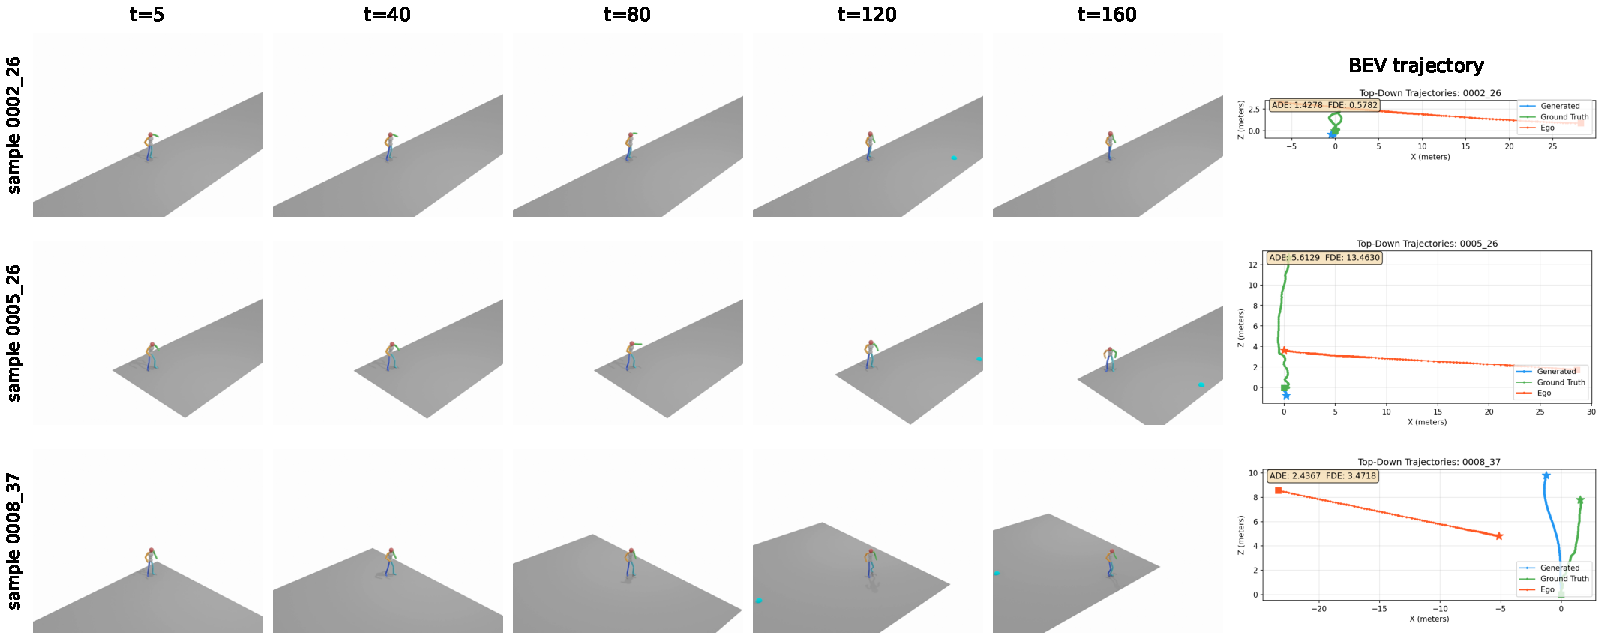
\includegraphics[width=\linewidth]{figures/qualitatives.pdf}
  \caption{Qualitative results from \method (epoch 3399, CFG=10) on three ego-conditioned samples from our test set. Each row shows five timesteps of the generated 3D body motion (HumanML3D, rendered as a rigged skeleton on a small ground plane) alongside a bird's-eye-view trajectory plot (rightmost column) showing the predicted pedestrian root trajectory (blue), ground-truth root trajectory (orange), and ego-vehicle trajectory (red). The root trajectory and orientation changes respond to the ego context. Note that the body pose inherits the limitations quantified in Sec.~\ref{sec:posequality}: the feet slide rather than plant, in the generated motion as in the labels.}
  \label{fig:qualitatives}
\end{figure*}

%----------------------------------------------------------------------
\section{Ablation Study}
\label{sec:ablation}
%----------------------------------------------------------------------

\subsection{Latent Dimension: 4 vs.\ 8}

To test whether a larger VAE latent space improves generation quality, we train a latent-8 VAE and ego-conditioned diffusion model (Latent-8).
As shown in Table~\ref{tab:main}, Latent-8 achieves FID $= 6.677$ — \textbf{19\% worse} than Pooled's 5.620 at the same epoch and CFG (unified evaluation).
R-Precision is essentially unchanged (Latent-8: 0.663 vs.\ Pooled: 0.665), confirming that the bottleneck for conditioning quality is the ego encoder, not the latent space.

The mechanism: the fixed-capacity denoiser must now model an 8D latent distribution instead of 4D, a strictly harder task, without any additional denoiser parameters.
The marginal diversity improvement (Diversity: 5.887 vs.\ 5.819, $+1.2\%$) does not compensate.
\textbf{Lesson}: increasing latent dimension is a poor lever for FID improvement without scaling the denoiser capacity proportionally.

\subsection{Interaction-Aware Sampling: a Training-Data 2$\times$2}
\label{sec:pipeline2x2}

The interaction-aware pipeline of Section~4.1 (score-weighted sampling + closest-approach cropping) is a training-\emph{data} intervention, orthogonal to the conditioning architecture.
We disentangle the two with a full 2$\times$2: each conditioning architecture (pooled, full-sequence) trained with and without the interaction pipeline, all evaluated under the unified pipeline. Table~\ref{tab:pipeline2x2} reports the four cells.

\begin{table}[t]
  \centering
  \caption{Training-data pipeline 2$\times$2 (FID $\downarrow$, unified eval, 3 replications; best checkpoint per cell). The two interventions are approximately additive: conditioning granularity dominates ($\approx$2.7--2.8 FID in both columns), and interaction-aware sampling contributes a similar absolute gain to both architectures ($-$0.59 pooled, $-$0.51 full-sequence).}
  \label{tab:pipeline2x2}
  \vspace{4pt}
  \begin{tabular}{lcc}
    \toprule
    & $-$ interaction sampling & $+$ interaction sampling \\
    \midrule
    Pooled        & 6.214 {\scriptsize $\pm$0.105} & 5.620 {\scriptsize $\pm$0.117} \\
    \method & 3.392 {\scriptsize $\pm$0.179} & \textbf{2.880} {\scriptsize $\pm$0.084} \\
    \bottomrule
  \end{tabular}
\end{table}

Two conclusions follow.
First, the conditioning-granularity gap ($\approx$2.7--2.8 FID in both columns) is roughly five times the pipeline effect, confirming that full-sequence conditioning — not data curation — is the primary driver.
Second, the two interventions are approximately additive: interaction-aware sampling contributes a similar absolute gain to both architectures ($-$0.59 pooled, $-$0.51 full-sequence), and for the full-sequence model the best checkpoint additionally arrives at $1/3$ the epochs.
The $+$pipeline full-sequence cell (\method-IA) has the best marginal of the four; \method remains the best-conditioned configuration (Sec.~\ref{sec:adefde}).

\subsection{Training-Seed Sensitivity}
\label{sec:seeds}

We retrain \method from two additional seeds under its original recipe and select each seed's best checkpoint by training-time validation FID (the same protocol as the main results).
Definitive best-checkpoint FID across the three seeds is $3.392$, $4.719$, and $4.803$ (mean $4.30 \pm 0.79$): the headline seed is markedly better than the other two, so single-seed point estimates in this setting overstate precision, and we report the spread explicitly.
The cross-\emph{architecture} conclusions are unaffected — every \method seed remains well below the pooled baseline (5.620), and the Pooled baseline itself proved training-unstable (two additional Pooled seeds were still above FID 10.9 when stopped at roughly 2{,}400 epochs, about half the epoch at which the reported seed peaked, at around four times lower throughput), meaning all our comparisons use the baseline's \emph{best} seed and are conservative in the baseline's favor.
Running the per-condition protocol on all three \method seeds sharpens the point considerably. While FID ranges over $3.392$--$4.803$ across those seeds, a relative spread of $33\%$, their trajectory error ranges only over $2.258$--$2.375$\,m ($5\%$) and their behavioural separation over $0.311$--$0.334$ ($7\%$). The per-condition instruments are several times more stable under reseeding than the metric the field reports, which is a further argument for reading conditioning off them. All three seeds beat the trained unconditional prior decisively and the pooled baseline significantly (paired bootstrap, $p \le 0.048$), so the per-condition ranking --- unlike the FID ranking --- does not depend on which seed we happened to report.
\method-IA, in contrast, \emph{replicates}: a second seed trained with an identical recipe and selected by the same rule reaches FID $2.671 \pm 0.031$ (its best-validation checkpoint is epoch 899) against the reported seed's $2.880 \pm 0.084$, i.e.\ a seed mean of $2.78 \pm 0.15$ --- a spread far tighter than \method's. The per-condition picture replicates as well: the second seed reaches ADE 2.63 and behavioural separation 0.13 (reported seed: 2.66 and 0.16), both short of \method (2.36 and 0.33), so \method-IA's weaker conditioning fidelity is a property of the interaction-sampling recipe rather than of one unlucky seed. At a matched epoch (1299) the second seed gives FID $3.320 \pm 0.139$, which shows that the two seeds reach their best marginal at different epochs and that per-seed checkpoint selection, not a fixed epoch, is the meaningful protocol.

\subsection{Encoder Freeze vs.\ Unfreeze}
\label{sec:h6}

The most important ablation is whether to freeze the ego encoder during diffusion training.
Unfrozen uses an identical architecture to \method but with the ego encoder left trainable, allowing the encoder to co-adapt with the denoiser via backpropagation through the diffusion loss.

Figure~\ref{fig:h6_training} shows the Unfrozen training trajectory (FID and R@1 vs.\ epoch).
Two behaviors are notable:
\begin{itemize}
  \item \textbf{FID/R@1 tradeoff}: As training progresses, R@1 improves (encoder specializes discriminatively) but FID degrades (generation quality decreases). The two optima do \emph{not} coincide: training-time FID is best at epoch 2099 (4.789), while R@1 continues rising long after FID has begun to deteriorate.
  \item \textbf{R@1 saturation far below \method}: After epoch $\approx$3299, training-time R@1 saturates, oscillating in the 0.37--0.42 band through epoch 4999 (maximum 0.417 at epoch 4599) while FID remains between 5.1 and 6.3. Neither metric ever approaches \method's operating point (FID 3.392, R@1 0.548) at any point in 5000 epochs.
\end{itemize}

Definitive evaluations (3 replications, CFG~=~10) confirm the picture, and are reported in Table~\ref{tab:h6}:

\begin{table*}[t]
  \centering
  \caption{Unfrozen definitive evaluation at three checkpoints. \method reference included for comparison.}
  \label{tab:h6}
  \vspace{4pt}
  \begin{tabular}{lcccc}
    \toprule
    System & FID $\downarrow$ & R@1 $\uparrow$ & MM $\uparrow$ & Diversity \\
    \midrule
    Unfrozen, epoch 2099 (best validation FID)      & 4.952 {\scriptsize $\pm$0.088} & 0.263 {\scriptsize $\pm$0.009} & 2.455 & 5.957 \\
    Unfrozen, epoch 3299 (best R@1)      & 5.311 {\scriptsize $\pm$0.060} & 0.348 {\scriptsize $\pm$0.004} & 2.581 & 6.034 \\
    Unfrozen, epoch 3399 (matched to \method)  & 5.079 {\scriptsize $\pm$0.034} & 0.352 {\scriptsize $\pm$0.009} & 2.618 & 6.064 \\
    \midrule
    \textbf{\method, epoch 3399 (frozen encoder)} & \textbf{3.392} {\scriptsize $\pm$0.179} & \textbf{0.548} {\scriptsize $\pm$0.002} & \textbf{3.956} & 5.794 \\
    \bottomrule
  \end{tabular}
\end{table*}

Unfrozen is worse than \method on FID, R-Precision and MultiModality at \emph{every} evaluated checkpoint (it is, however, slightly better on mean trajectory error; Sec.~\ref{sec:adefde}).
Later checkpoints cannot change this conclusion: even Unfrozen's best training-time R@1 in the saturation band (0.417 at epoch 4599, with training-time FID 6.339) remains far below \method's definitive R@1 of 0.548 — and training-time metrics consistently \emph{overestimate} the definitive 3-replication values (\eg 0.398~$\to$~0.348 at epoch 3299).
The MultiModality collapse is particularly striking: Unfrozen MM $= 2.618$ vs.\ \method MM $= 3.956$ (34\% lower).
This indicates near-deterministic generation per condition — the ego encoder has learned highly discriminative features for each trajectory, collapsing the generated motion distribution to a narrow region.

\paragraph{Mechanism.}
When the encoder is frozen (\method), it maps ego trajectories to general-purpose representations aligned with the VAE latent space.
The denoiser learns to query these fixed representations and generate diverse, plausible motions for each condition.
When the encoder is unfrozen (Unfrozen), backpropagation through the denoising loss pushes the encoder toward representations that \emph{minimize the denoising loss} — essentially learning discriminative features that uniquely identify each trajectory.
This over-specialization constrains generation: the denoiser outputs similar samples for each unique ego representation, collapsing MultiModality.

This pattern mirrors the frozen-encoder paradigm in image generation~\cite{rombach2022sd,ye2023ipadapter,zhang2023controlnet}: frozen conditioning encoders preserve general-purpose representations and allow the generative model to learn diverse ways to satisfy the conditioning signal.

\begin{figure}[t]
  \centering
  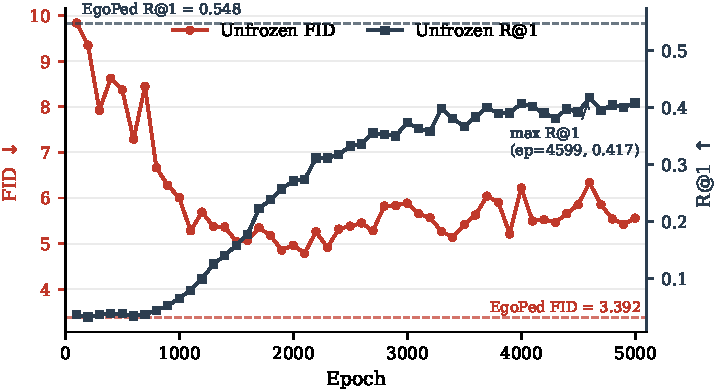
\includegraphics[width=0.9\linewidth]{figures/h6_training_curve.pdf}
  \caption{Unfrozen training trajectory: training-time validation FID (left axis, red) and R@1 (right axis, blue) vs.\ epoch, over the full 5000-epoch run. FID is best at epoch~2099 and degrades as R@1 rises; after epoch~$\approx$3299, R@1 saturates in the 0.37--0.42 band while FID oscillates between 5.1 and 6.3. Dashed reference lines show \method's best operating point (FID=3.392, R@1=0.548 at epoch 3399, CFG 10). Unfrozen never approaches \method's performance on either metric.}
  \label{fig:h6_training}
\end{figure}

\paragraph{Is the pretraining necessary?}
Freezing alone is not sufficient: an \method model trained with a \emph{randomly initialized} frozen ego encoder (identical otherwise) reaches only FID $= 4.968 \pm 0.171$ with R-Precision@1 exactly at chance — statistically indistinguishable from the ego-zeroed null branch (FID $5.18$, Table~\ref{tab:trivial}) --- though that branch is itself a weak reference, and a properly trained prior reaches 3.24, so the random-encoder model is worse than simply not conditioning at all.
Together with Unfrozen, this brackets the design from both sides: the alignment pretraining is what \emph{injects} usable ego information, and freezing is what \emph{preserves} generative diversity while using it.

\subsection{Conditioning Mechanism: Self-Attention vs.\ Cross-Attention}
\label{sec:xattn}

Our denoiser injects the ego sequence by concatenating it with the latent tokens and applying self-attention over the joint sequence (Section~\ref{sec:experiments}).
A common alternative for sequence conditioning is \emph{cross-attention}, where the latent tokens act as queries and the ego sequence as keys and values, so the ego tokens never attend among themselves and the attention cost is $\mathcal{O}(L\times T)$ rather than $\mathcal{O}((L+T)^2)$.
To test whether the specific mechanism matters, we train an otherwise-identical cross-attention denoiser (same frozen VAE and frozen ego encoder, same data, same effective batch size) and evaluate it on the held-out test split.

\begin{table*}[t]
  \centering
  \caption{Conditioning-mechanism ablation. Both denoisers consume the full 196-token ego sequence and differ only in how they attend to it. Evaluated on the held-out test split (a scene-disjoint half of the validation set), CFG~=~10, mean~$\pm$~95\% CI over 3 replications, best checkpoint each. The two mechanisms are statistically comparable (overlapping FID intervals); cross-attention provides no advantage. The intervals here are over sampling replications at one training seed per arm, and \method's seed spread ($\pm0.79$, Sec.~\ref{sec:seeds}) is far wider, so this comparison can exclude a large effect but cannot resolve a small one.}
  \label{tab:xattn}
  \vspace{4pt}
  \small
  \begin{tabular}{lcccc}
    \toprule
    Denoiser & Attention over ego & FID $\downarrow$ & R@1 $\uparrow$ & MM $\uparrow$ \\
    \midrule
    Self-attention (\method) & concatenation      & \textbf{3.338} {\scriptsize $\pm$0.190} & \textbf{0.537} & 4.14 \\
    Cross-attention          & queries/keys-values & 3.490 {\scriptsize $\pm$0.059} & 0.501 & \textbf{4.61} \\
    \bottomrule
  \end{tabular}
\end{table*}

As shown in Table~\ref{tab:xattn}, the self-attention and cross-attention denoisers achieve statistically comparable FID (3.338 vs.\ 3.490; 95\% CIs $[3.15, 3.53]$ and $[3.43, 3.55]$ overlap), with self-attention holding a slight edge on retrieval alignment (R@1) and cross-attention generating marginally more diverse motion per condition (MM).
Note that the comparison is, if anything, generous to the cross-attention variant: its best checkpoint was selected on the held-out split itself, whereas the self-attention model's checkpoint was fixed in advance from training-time validation.
We also observed that the cross-attention variant trained less stably, with a noisier FID-vs-epoch trajectory.
\textbf{Takeaway}: the large improvement over pooled conditioning (Table~\ref{tab:main}) comes from exposing the denoiser to the \emph{full} per-timestep ego sequence, not from any particular attention mechanism -- either self-attention over the concatenated sequence or cross-attention works, and neither is required over the other.

\subsection{Checkpoint Selection}

A non-obvious finding (relevant to practitioners) is that FID does not monotonically improve with training.
Pooled's epoch trajectory shows FID $= 6.603$ at epoch 4399, FID $= 8.400$ at epoch 4599 (regression), and FID $= 7.510$ at epoch 4999 (partial recovery) — despite flat training loss throughout.
\method similarly peaks at epoch 3399 (definitive FID $= 3.392$) and degrades steadily thereafter (Fig.~\ref{fig:h4_training}).
\textbf{Lesson}: the final checkpoint is not the best checkpoint. Periodic FID validation during training is essential; early stopping on FID is critical.

\begin{figure}[t]
  \centering
  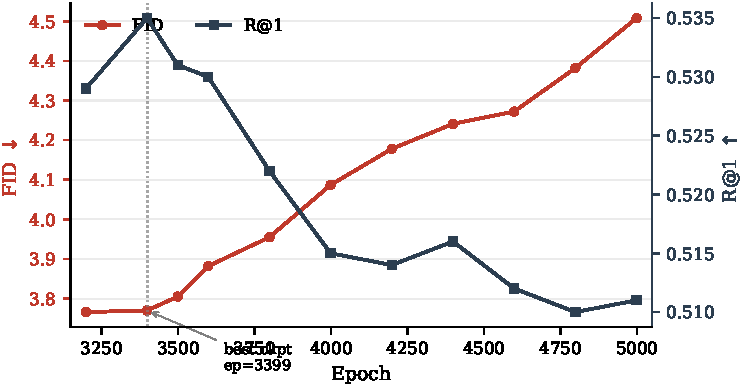
\includegraphics[width=0.9\linewidth]{figures/h4_training_curve.pdf}
  \caption{\method training trajectory: training-time validation FID (left axis, red) and R@1 (right axis, blue) across the late training segment. Epoch~3399 is the best checkpoint (highest R@1, FID within noise of epoch~3199, and best definitive 3-replication FID); both metrics then degrade steadily through epoch~4999. Training loss is flat across this range — sampling quality oscillates independently of training loss.}
  \label{fig:h4_training}
\end{figure}

%----------------------------------------------------------------------
\section{Discussion}
\label{sec:discussion}
%----------------------------------------------------------------------

\paragraph{Architecture recommendation.}
The experimental evidence strongly favors the \method architecture: frozen ego encoder + full-sequence conditioning denoiser (self-attention over the concatenated latent and ego sequence; cross-attention works equally well, Section~\ref{sec:xattn}).
Future work seeking to improve conditioning fidelity should explore adapter-style approaches — fine-tuning a lightweight adapter on the frozen encoder while keeping the backbone fixed — rather than end-to-end unfreezing.

\paragraph{R-Precision@1 and the conditioning-diversity tradeoff.}
\method's R@1 (0.548) is lower than Pooled's (0.665) despite dramatically better FID.
We caution against reading this as a conditioning deficit. R@1 is computed in the ego encoder's own alignment space, and each model is scored in the space its own encoder induces, so the measure is not comparable across models with differently trained encoders; the per-condition metrics of Secs.~\ref{sec:adefde} and \ref{sec:behavior}, which use no learned embedding, rank \method above Pooled on both axes.
In AV simulation this is desirable: a single ego trajectory should plausibly lead to several pedestrian behaviours (crossing, waiting, accelerating).
A genuine tradeoff is present too: full-sequence conditioning generates more diverse motions per condition, which spreads the embedding distribution and lowers retrieval accuracy.

\paragraph{Broader impact.}
The primary intended use of ego-conditioned pedestrian motion generation is autonomous-driving simulation: synthesizing realistic, ego-aware pedestrian behaviors enables larger-scale safety testing without exposing real pedestrians to risk, and is particularly valuable for the long tail of rare or safety-critical interactions that are unsafe or impractical to collect.
We note two risks.
First, generated pedestrian motions could in principle be used adversarially, e.g.\ to seed motion-planning policies that learn to expect only nominal behaviors and consequently fail on out-of-distribution pedestrians; we mitigate this by reporting MultiModality and diversity metrics, which expose the breadth of the generated distribution rather than only its mean.
Second, training data inherit demographic biases of the source AV datasets (AVA, nuScenes, Waymo): generated motion is conditioned on the distribution of pedestrians actually observed in U.S./European urban environments, so deployment in other settings should be preceded by additional validation.
Generated motion data is synthetic and contains no personally identifiable information.


%----------------------------------------------------------------------
\section{Limitations and Future Work}
\label{sec:limitations}
%----------------------------------------------------------------------

\begin{itemize}
  \item \textbf{Body pose quality}: Pedestrian poses are estimated (not ground-truth 3D), and Sec.~\ref{sec:posequality} quantifies the cost: a single canonical skeleton for every pedestrian (no body-shape variation), a median foot-skate ratio of 0.97 with $94.6\%$ of moving sequences never planting a foot, and root-relative joint variability at $0.44\times$ real mocap. The root trajectories are reliable; the body is a lightly articulated template sliding along them. Direct 3D body annotation from datasets like JRDB-Pose or BEDLAM, or a physics-based refit of the existing labels, would address this, and we regard it as the single largest quality constraint on the benchmark.
  \item \textbf{Conditioning scope}: We condition only on 2D ego trajectory. Incorporating relative pedestrian-ego geometry, ego velocity profile, or map elements could improve fidelity.
  \item \textbf{R-Precision is not cross-model comparable}: \method scores 0.548 against Pooled's 0.665, but each model is evaluated in its own encoder's alignment space, so we do not treat this as evidence about conditioning; it is reported for completeness and the evaluator-independent metrics are used instead.
  \item \textbf{Physics}: Generated motions are not physically constrained (foot sliding, penetration). This is inherited as well as produced --- the training labels themselves slide (Sec.~\ref{sec:posequality}) --- so a model that reproduces the data faithfully will reproduce the sliding. Post-hoc physics cleanup, or a contact-aware loss, could improve realism for simulation deployment.
  \item \textbf{Evaluator domain shift}: FID and Diversity rely on motion-feature encoders pretrained on HumanML3D, whose motion distribution differs from in-the-wild pedestrian motion; absolute FID values should be compared only within our benchmark. The target distribution is also damped relative to mocap (Sec.~\ref{sec:posequality}), which makes the marginal easier to fit than pose realism alone would imply --- a second reason not to read FID as a realism score.
  \item \textbf{Single benchmark, no perceptual study}: All results are on our combined AVA/nuScenes/Waymo benchmark, and we do not yet report a human perceptual study of motion realism.
\end{itemize}

\paragraph{Future work.}
The pose audit of Section~\ref{sec:posequality} defines the most consequential next step. Our de-sliding pilot shows that contact-corrected labels are representable by the motion autoencoder after fine-tuning, which scopes the remedy as a relabelling and retraining effort rather than an additional generation-time loss. Carrying it out would invalidate every distributional number reported here, since it changes the target distribution itself, and we therefore treat it as a separate undertaking rather than a revision of these results. Beyond the labels, three extensions follow directly from our findings. Richer conditioning --- relative pedestrian--vehicle geometry, ego velocity profile, or map topology --- is a natural way to raise the information content of the condition beyond the $196\times2$ trajectory. A human perceptual study would supply the realism judgement that no distributional score on these labels can provide. Finally, the dissociation we document motivates a per-condition benchmark protocol for conditional motion generation in general: our trajectory-error and behavioural-coupling probes are a minimum, and more discriminating conditioning tests are an open problem.

%----------------------------------------------------------------------
\section{Conclusion}
%----------------------------------------------------------------------

We introduced \method, an ego-conditioned pedestrian body motion generation system based on latent diffusion with full-sequence ego conditioning.
Our key finding is that exposing the denoiser to the full 196-token ego trajectory sequence dramatically outperforms single-token pooled conditioning: a 40\% FID improvement (5.620~$\to$~3.392) under a unified evaluation pipeline, with non-overlapping confidence intervals, verified on a scene-disjoint held-out split, on evaluator-independent trajectory metrics, and conservative with respect to both training-data curation and baseline seed selection. Our second finding qualifies how such numbers should be read: because a well-trained unconditional model matches that FID, and one trained with interaction-aware sampling beats every conditional model at 1.43 while ignoring the vehicle entirely, FID ranks marginals rather than conditioning. The claim that the ego trajectory is used rests instead on per-condition trajectory error and on the coupling of generated stopping decisions to the vehicle, where full-sequence conditioning leads. Interaction-aware data sampling improves the marginal to FID = 2.880 (2.67--2.88 over two seeds) but not per-condition fidelity.
A paired ablation reveals that frozen ego encoders are critical: unfreezing causes 34\% MultiModality collapse as the encoder over-specializes to discriminative features.

These results establish a clear design recipe for ego-conditioned motion generation in AV settings:
pretrain the ego encoder to regress frozen VAE latents, then freeze it during diffusion training and condition the denoiser on the full ego sequence.
This recipe is the best-conditioned configuration we found across AVA, nuScenes, and Waymo, and provides a foundation for scalable, behavior-consistent pedestrian simulation.

%----------------------------------------------------------------------
\bibliographystyle{IEEEtran}
\bibliography{refs}
%----------------------------------------------------------------------

%----------------------------------------------------------------------
\appendices
%----------------------------------------------------------------------

\section{Unfrozen-Encoder Training Trajectory}
\label{app:h6_trajectory}

Table~\ref{tab:h6_trajectory} lists the training-time validation metrics behind Figure~\ref{fig:h6_training}, at the checkpoint evaluation points referenced in Section~\ref{sec:h6}.

\begin{table}[t]
  \centering
  \caption{Unfrozen: training-time validation metrics at selected checkpoint evaluation points (validation runs every 100 epochs; full curve in Figure~\ref{fig:h6_training}).
           Training-time FID is best at epoch 2099 (4.789); R@1 rises until epoch $\approx$3299, then saturates in the 0.37--0.42 band (maximum 0.417 at epoch 4599) while FID remains between 5.1 and 6.3.}
  \label{tab:h6_trajectory}
  \vspace{4pt}
  \begin{tabular}{ccc}
    \toprule
    Epoch & Train-time FID $\downarrow$ & Train-time R@1 $\uparrow$ \\
    \midrule
    99    & 9.835 & 0.036 \\
    499   & 8.373 & 0.038 \\
    999   & 6.011 & 0.065 \\
    1499  & 5.053 & 0.158 \\
    1999  & 4.967 & 0.271 \\
    \textbf{2099}  & \textbf{4.789} & 0.273 \\
    2499  & 5.385 & 0.332 \\
    2999  & 5.889 & 0.373 \\
    3299  & 5.273 & 0.398 \\
    3399  & 5.141 & 0.380 \\
    3499  & 5.415 & 0.367 \\
    3999  & 6.221 & 0.407 \\
    \textbf{4599}  & 6.339 & \textbf{0.417} \\
    4999  & 5.561 & 0.408 \\
    \bottomrule
  \end{tabular}
\end{table}

\end{document}
